\documentclass[a4paper,12pt]{article}  % 14pt for a 2-size larger font
\usepackage[utf8]{inputenc}
\usepackage{graphicx}
\usepackage{array}
\usepackage{caption}
\usepackage{xcolor}
\usepackage{listings}
\usepackage{hyperref}
\usepackage{amsmath}
\usepackage[most]{tcolorbox}
\usepackage[margin=0.8in]{geometry} 
\usepackage{sectsty} % For section coloring
\usepackage{hyperref}

\hypersetup{
    colorlinks=true,
    linkcolor=violet,
    filecolor=magenta,      
    urlcolor=cyan,
}

% Define colors
\definecolor{codebg}{rgb}{0.95,0.95,0.95}
\definecolor{commentgreen}{rgb}{0.0,0.5,0.0}
\definecolor{keywordcolor}{rgb}{0.0,0.0,1.0}
\definecolor{stringcolor}{rgb}{1.0,0.0,0.0}
\definecolor{sectionbrown}{rgb}{0.65,0.16,0.16}
\definecolor{subsectiongreen}{rgb}{0.0,0.5,0.0}
\definecolor{subsubsectionpink}{rgb}{1.0,0.08,0.58}

% Style definitions for sections
\sectionfont{\color{sectionbrown}}


% Define a custom color
\definecolor{boldblue}{rgb}{0.0, 0.0, 1.0}

% Redefine \textbf to apply both bold and color
\renewcommand{\textbf}[1]{\textcolor{violet}{\bfseries #1}}



\lstdefinestyle{mystyle}{
    backgroundcolor=\color{codebg},
    basicstyle=\ttfamily\footnotesize,
    commentstyle=\color{commentgreen},
    keywordstyle=\color{keywordcolor},
    stringstyle=\color{stringcolor},
    frame=single,
    tabsize=4,
    showstringspaces=false,
    captionpos=b,
    breaklines=true,
    breakatwhitespace=false,
}

\lstset{style=mystyle}

% Define a tcolorbox style for text with border
\tcolorboxenvironment{quote}{
    colback=yellow!10,
    colframe=blue!75!black,
    fonttitle=\bfseries,
    colbacktitle=blue!10,
    title=Problem Description,
}



\begin{document}

% Title Page
\begin{titlepage}

\begin{figure}[h]
    \centering
    \includegraphics[width=0.3\textwidth]{cu.png}
\end{figure}

\vspace{1cm}

\noindent
\begin{tabular}{@{}p{\textwidth}@{}}
    \hline
    \hline
    \vspace{0.2cm}
    \begin{center}
        \Huge{\textbf{Movie Management System}} % Insert your project title here
    \end{center}
    \vspace{0.2cm}\\
    \hline
    \hline
\end{tabular}

\vspace{4cm}

\begin{center}
    {\large Database Project Report} % Document type (e.g., Project Report)
    \\
    {\Large Group-66} % Insert group number
\end{center}

\vfill

\begin{center}
    Report submitted 14 December, 2024
\end{center}

\vfill

\noindent A project submitted to \textbf{Dr. Rudra Pratap Deb Nath}, Associate Professor, Department of Computer Science and Engineering, Chittagong University (CU), in partial fulfillment of the requirements for the Database Systems Lab course. The project is not submitted to any other organization at the same time.

\end{titlepage}
\clearpage

% Group Details Table
\begin{table}[t]
\centering
\caption{Details of Group-XX} % Insert your group number
\resizebox{\textwidth}{!}{%
\begin{tabular}{|l|l|l|l|l|}
\hline
Roll ID & Name & Signature & Date & Supervisor Approval\\
\hline
22701066 & Tanjim Tajwar Arnab & \includegraphics[width=2cm]{sign.jpg} & 14-12-2024 & \\
\hline
      
\end{tabular}%
}

\end{table}
\clearpage

% Table of Contents
\tableofcontents
\clearpage

% Abstract
\begin{abstract}
\noindent The Movie Management System is a comprehensive full-stack web application designed to streamline the process of movie ticket bookings and enhance the movie-going experience. The platform allows users to sign up, log in, view showtimes, book or purchase tickets for movies, browse upcoming movie releases, cancel bookings, and leave reviews for watched movies. By addressing the need for a centralized and user-friendly movie management platform, this system empowers users to manage their movie preferences effortlessly.  

Additionally, the platform includes robust administrative functionalities, enabling administrators to oversee and manage user accounts, review user bookings, monitor reviews provided by users, and delete user information or bookings if necessary. With a carefully crafted database design, the application ensures efficient data processing and scalability. The Movie Management System distinguishes itself with its interactive features, intuitive interface, and reliable functionalities, making it a valuable tool for both users and cinema administrators. Future developments may include personalized movie recommendations and improved analytics for administrators to enhance the overall experience.
\end{abstract}


\clearpage

% Introduction


\section{Introduction} \label{sec:introduction}
\noindent The objective of this course is to develop a database application system by applying the theories, methodologies, tools, and technologies learned in \textit{[Insert course code and name]}.  

\begin{itemize}
    \item \textbf{Background and Motivation:}  
    The Movie Management System was conceived to address the following challenges:  
    \begin{itemize}
        \item Lack of a centralized platform for users to manage movie bookings efficiently.  
        \item Difficulty in accessing reliable information about upcoming movies and showtimes.  
        \item Fragmented and inconsistent user experiences across existing solutions.  
        \item Inadequate administrative features for managing bookings, user accounts, and reviews.  
    \end{itemize}  
    By building this system, we aim to provide a seamless and user-friendly platform for moviegoers, while empowering administrators with robust tools for efficient management.  

    \item \textbf{Problem Statement:}  
    The Movie Management System addresses these specific problems:  
    \begin{itemize}
        \item Users face challenges in viewing showtimes, booking or purchasing tickets, and canceling bookings.  
        \item Limited functionality in existing platforms for leaving or accessing reliable movie reviews.  
        \item Administrators lack comprehensive tools to oversee user accounts, manage bookings, and moderate reviews effectively.  
    \end{itemize}  
    Key entities include:  
    \begin{itemize}
        \item \textbf{Users:} To book tickets, view showtimes, cancel bookings, and provide reviews.  
        \item \textbf{Movies:} To manage details like showtimes, upcoming releases, and reviews.  
        \item \textbf{Showtimes:} To enable users to select preferred movie schedules.  
        \item \textbf{Reviews:} To allow users to share feedback on movies they have watched.  
    \end{itemize}  

    \item \textbf{System Definition:}  
    The Movie Management System provides:  
    \begin{itemize}
        \item A user interface for moviegoers to browse showtimes, book tickets, cancel bookings, and review movies.  
        \item Administrative functionalities to manage user accounts, oversee reviews, and monitor bookings.  
        \item Scalability for future enhancements, including personalized movie recommendations and analytics tools for administrators.  
    \end{itemize}  




 
 \item \textbf{System Development Process:} The system development process involves the following steps:
 Project Management → Requirement Gathering and Analysis → System Design → Implementation → Validation → Testing → Deployment → Maintenance and Enhancement → Documentation.

     
\end{itemize}


\clearpage



% Project Management
\section{Project Management} \label{sec:projectmanagement}


Effective project management was crucial for the success of the Movie Management System project, even though the project was developed by a single individual, Tanjim Tajwar Arnab. As the sole developer, Tanjim managed all aspects of the project, ensuring efficient resource use, maintaining clear communication with self, and guaranteeing timely delivery of milestones. The following subsections outline the key components of the approach taken:

\subsection{Roles and Responsibilities}
Although the project was developed by one person, the roles and responsibilities typically distributed across a team were all handled by Tanjim, who leveraged their expertise to ensure that every aspect of the project was meticulously addressed:

\begin{itemize}
    \item \textbf{Project Manager and Developer}: As the sole individual responsible for the Movie Management System, Tanjim took on the role of Project Manager and Developer. Tanjim oversaw the entire development process, from planning and resource management to execution. They coordinated all tasks, handled coding and debugging, tracked progress against milestones, and ensured that the project stayed on schedule. This included managing the frontend (using HTML, CSS, and PHP) and backend (PHP, SQL, and XAMPP) components of the system, as well as taking care of database administration and testing. Tanjim also handled the project's design aspects, ensuring that the application was visually appealing, user-friendly, and functional.
    
    \item \textbf{Frontend Development}: Tanjim was responsible for creating the user interface (UI) of the Movie Management System, which included designing and implementing elements such as booking tickets, browsing movie showtimes, and viewing upcoming movies. Using HTML, CSS, and PHP, Tanjim created a responsive, visually appealing, and functional application that offered a seamless user experience.
    
    \item \textbf{Backend Development}: Tanjim managed the server-side development of the Movie Management System, handling tasks such as the logic for managing user bookings, movie schedules, and payment processes. Using PHP, PHPMyAdmin, and SQL, Tanjim ensured that data was securely stored, and processes like payments and bookings ran smoothly. XAMPP was used for local server development to simulate real-world deployment conditions.
    
    \item \textbf{Database Administration}: Tanjim also handled database administration tasks, including designing the database structure using MySQL and PHPMyAdmin. They implemented the schema, ensured data integrity, and optimized the database to handle user bookings, movie schedules, and user reviews. Backup and recovery procedures were also set up to secure data.
    
    \item \textbf{Quality Assurance (QA) Testing}: As the sole developer, Tanjim was responsible for testing the Movie Management System to ensure that all features, including the booking functionality, payment system, and review submissions, worked without issues. They identified and fixed bugs, conducted performance testing, and ensured the system could handle high traffic during peak hours.
    
    \item \textbf{Scrum Practices and Project Management}: Tanjim also took on the role of Scrum Master by implementing Scrum practices and agile methodologies to structure the workflow. They organized personal work sprints, tracked the backlog, set deadlines, and ensured continuous improvement by managing personal feedback loops.
\end{itemize}


\subsection{Tools Used}
To effectively manage and execute the project, a range of tools were utilized that supported development, testing, and documentation. These tools helped streamline the workflow and ensured efficient project execution.

\begin{itemize}
    \item \textbf{GitHub}: \textbf{GitHub} served as the version control system, allowing the project to be managed effectively. It enabled Tanjim to track changes, commit code, and maintain backups. GitHub also facilitated code reviews, issue tracking, and the organization of project documentation.
    
    \item \textbf{VSCode}: \textbf{Visual Studio Code} (VSCode) was the primary code editor used for development. It provided a lightweight, customizable environment with extensions to support HTML, CSS, PHP, and SQL. VSCode's integrated terminal, syntax highlighting, and debugging tools enhanced the efficiency of writing and testing code.
    
    \item \textbf{Chrome}: \textbf{Google Chrome} was used for testing and debugging the Movie Management System. It allowed Tanjim to view and interact with the application, ensuring the UI was responsive and functioning as intended. Chrome’s developer tools were crucial for inspecting elements, troubleshooting, and testing performance across different devices and screen sizes.
    
    \item \textbf{Frontend}: \textbf{HTML, CSS, PHP} were used for the frontend development of the system. These technologies helped build the user interface (UI) that was both visually appealing and responsive.
    
    \item \textbf{Backend}: \textbf{PHP, PHPMyAdmin, SQL, and XAMPP} were used for backend development. PHP handled the server-side logic, while PHPMyAdmin and SQL were used for managing and interacting with the database. XAMPP was used to set up a local server environment.
    
    \item \textbf{Report}: The project report was created using \textbf{Overleaf}, a LaTeX editor that helped generate professional-looking reports with precise formatting.
    
    \item \textbf{Resources}: Information for the project was gathered from various online platforms, including \textbf{GitHub, YouTube, W3Schools}, and other websites. These resources were essential for learning, problem-solving, and finding solutions to challenges encountered during the project.
    
    \item \textbf{Images}: Images for the project were sourced from \textbf{Pinterest}, which provided a collection of visuals to enhance the overall design of the Movie Management System.
\end{itemize}


\subsection{Scrum Methodology}
The Movie Management System project was managed using the Scrum methodology, an Agile framework that emphasizes collaboration, flexibility, and iterative progress. Scrum allowed the project to adapt to changing requirements, deliver value incrementally, and maintain a high level of communication throughout the development process. The following key Scrum ceremonies and practices were essential to the project’s success:

\begin{itemize}
    \item \textbf{Sprint Planning}: At the beginning of each sprint, a Sprint Planning meeting was held to define the sprint goals, identify high-priority tasks, and select features for completion. The tasks were estimated based on their complexity and the available time in the sprint (usually 2-3 weeks). As the sole developer, Tanjim was responsible for estimating the effort required and ensuring that each task was achievable within the sprint timeline.
    
    \item \textbf{Daily Stand-ups}: Even as a single developer, daily stand-ups were held to reflect on the progress made the previous day, set goals for the current day, and identify any obstacles or challenges. These brief meetings helped maintain focus, ensure accountability, and identify areas where adjustments were necessary. Although the team was small, this practice kept the workflow organized and on track.
    
    \item \textbf{Sprint Review}: At the end of each sprint, a Sprint Review was conducted to assess the work completed during the sprint. The completed features were tested and reviewed, and feedback was collected to ensure that the project met the requirements and user needs. This meeting provided an opportunity to demonstrate progress and adjust any priorities or objectives for the next sprint.
    
    \item \textbf{Sprint Retrospective}: After the Sprint Review, a Sprint Retrospective was held to reflect on the development process. The focus was on identifying areas for improvement, such as optimizing development workflows or overcoming challenges faced during the sprint. The retrospective allowed for continuous improvement and provided insights that enhanced the overall quality of the project.
\end{itemize}

By following Scrum practices, the Movie Management System project was able to maintain flexibility, adapt to changes efficiently, and continually improve throughout development. The iterative nature of Scrum ensured that value was delivered incrementally, with each sprint contributing to the overall completion of the system. This approach ultimately led to the successful delivery of the Movie Management System, on time and in line with project goals.





\clearpage





    \section{Process of Requirement Gathering and Analysis}




\subsection{Discussion with Our Customer,Ticket Sellers, Movie Providers and Office Staff}
\subsubsection*{Discussion with Our Customer}
The objective of this discussion was to gather detailed information about the end-user requirements and expectations for the movie management system, particularly for ticket purchasing and movie reviews.

\textbf{Key Points Discussed:}
\begin{itemize}
    \item \textbf{Ticket Purchase Flow:} Customers want an easy and quick ticket booking system with features like selecting movie shows, choosing seats, and completing secure payments.
    \item \textbf{Review System:} Customers expect the ability to submit movie reviews, rate movies, and read others' reviews to help in movie selection decisions.
    \item \textbf{User Interface:} A user-friendly interface with clear navigation, filtering options by genre, movie ratings, and showtimes was emphasized.
    \item \textbf{Account Management:} Customers expressed a desire for easy login/signup options, ticket history tracking, and managing personal preferences.
\end{itemize}

\subsubsection*{Discussion with Ticket Sellers}
The objective was to understand the requirements and challenges faced by ticket sellers in managing and selling tickets for movies.

\textbf{Key Points Discussed:}
\begin{itemize}
    \item \textbf{Ticket Availability and Management:} Ticket sellers need a way to update the availability of tickets for different showtimes, handle cancellations, and provide refunds when necessary.
    \item \textbf{Transaction Processing:} A secure, efficient payment gateway is required to ensure smooth ticket purchases.
    \item \textbf{Notifications:} Ticket sellers need a system to notify customers of successful bookings, cancellations, or reschedules of movie tickets.
    \item \textbf{Analytics:} Ticket sellers require reports on ticket sales, popular movies, peak times, etc., to better manage inventory and optimize movie showings.
\end{itemize}

\subsubsection*{Discussion with Movie Providers}
The objective was to gather insights from movie providers regarding the information required for the movie management system and how the system can be designed to display movies effectively.

\textbf{Key Points Discussed:}
\begin{itemize}
    \item \textbf{Content Management:} Movie providers emphasized the need for a system to upload and update movie details, such as movie posters, trailers, descriptions, release dates, and cast information.
    \item \textbf{Promotion Management:} Providers requested the ability to promote special offers, discounts, and upcoming releases on the platform.
    \item \textbf{Showtime Management:} Providers need a way to define movie schedules for multiple theaters and locations.
    \item \textbf{Rights and Licensing:} Movie providers need a secure way to manage access to movie content and prevent unauthorized use or piracy.
\end{itemize}

\subsubsection*{Discussion with Office Staff}
The objective was to understand the administrative requirements for managing the movie system, including backend operations and support.

\textbf{Key Points Discussed:}
\begin{itemize}
    \item \textbf{Admin Panel:} Office staff will need access to a robust admin panel to manage user accounts, ticket sales, movie content, and reviews.
    \item \textbf{Monitoring and Reporting:} Staff need tools to track sales data, movie performance, and user reviews to ensure the system runs smoothly.
    \item \textbf{Customer Support:} An integrated customer support system for resolving issues like ticket problems, login issues, and payment disputes is essential.
    \item \textbf{System Maintenance:} Office staff emphasized the need for easy-to-use features to update movie listings, manage backend configurations, and ensure smooth system operation.
\end{itemize}


\subsection{Purpose of the System}

The Movie Management System aims to provide an efficient platform for managing movies, sessions, ticket sales, and user reviews. It serves administrators, customers, and moviegoers by streamlining operations such as scheduling movies, purchasing tickets, and reviewing films.

\subsection{Stakeholders}

\begin{enumerate}
    \item \textbf{Admin}
    \begin{itemize}
        \item Manages halls, movies, and sessions.
        \item Monitors ticket sales and user reviews.
    \end{itemize}
    
    \item \textbf{Customers (Viewers)}
    \begin{itemize}
        \item Browse movies and sessions.
        \item Purchase tickets.
        \item Submit reviews for watched movies.
    \end{itemize}
    
    \item \textbf{System Owner}
    \begin{itemize}
        \item Ensures system reliability and availability.
        \item Manages operational and security requirements.
    \end{itemize}
\end{enumerate}

\subsection{Functional Requirements}

\begin{enumerate}
    \item \textbf{User Management}
    \begin{itemize}
        \item Register new users.
        \item Login and logout functionality.
        \item Role-based access (Admin, Viewer).
    \end{itemize}
    
    
    \item \textbf{Movie Management (Admin)}
    \begin{itemize}
        \item Add, update, and delete movies.
        \item View movie details (title, genre, release date, duration, language).
    \end{itemize}
    
    
    \item \textbf{Ticket Management}
    \begin{itemize}
        \item Customers can view available sessions and select seats.
        \item Ticket purchase functionality.
        \item Ticket cancellation and refund policy.
    \end{itemize}
    
    \item \textbf{Review System}
    \begin{itemize}
        \item Customers can submit reviews for watched movies.
        \item View aggregated ratings and comments for each movie.
    \end{itemize}
    
    \item \textbf{Reporting and Analytics (Admin)}
    \begin{itemize}
        \item View ticket sales reports.
        \item Analyze movie popularity based on reviews and sales.
    \end{itemize}
\end{enumerate}

\subsection{Non-Functional Requirements}

\begin{enumerate}
    \item \textbf{Performance}
    \begin{itemize}
        \item The system should handle up to 1,000 concurrent users.
        \item Response time for key operations (e.g., ticket booking) should be under 2 seconds.
    \end{itemize}
    
    \item \textbf{Scalability}
    \begin{itemize}
        \item The system should support the addition of new halls and increased user traffic without significant performance degradation.
    \end{itemize}
    
    \item \textbf{Security}
    \begin{itemize}
        \item Role-based access control to restrict unauthorized actions.
    \end{itemize}
    
    \item \textbf{Usability}
    \begin{itemize}
        \item Intuitive user interface for both admins and customers.
        \item Accessible via desktop and mobile devices.
    \end{itemize}
    
    \item \textbf{Availability}
    \begin{itemize}
        \item System uptime of 99.9\%.
        \item Backup and disaster recovery plans.
    \end{itemize}
    
    \item \textbf{Compliance}
    \begin{itemize}
        \item Adherence to data privacy regulations (e.g., GDPR, CCPA) for user data.
    \end{itemize}
\end{enumerate}

\subsection{Use Cases}

\begin{enumerate}
    \item \textbf{Customer Use Cases}
    \begin{itemize}
        \item Search for movies and sessions.
        \item Purchase tickets for a selected session.
        \item Submit a review for a movie.
    \end{itemize}
    
    \item \textbf{Admin Use Cases}
    \begin{itemize}
        \item Manage movies, and sessions.
        \item Generate reports on sales and reviews.
    \end{itemize}
\end{enumerate}

\subsection{Data Requirements}

\begin{enumerate}
    \item \textbf{User Data}
    \begin{itemize}
        \item \textbf{Username}: A unique identifier for each user (Primary Key in \texttt{AccountUser} table).
        \item \textbf{Email}: A unique email address used for user identification and communication (Unique in \texttt{AccountUser} table).
        \item \textbf{Name}: The full name of the user (Stored in \texttt{AccountUser} table).
        \item \textbf{Phone}: The contact phone number of the user (Stored in \texttt{AccountUser} table).
        \item \textbf{Password}: A secure password for user login (Stored in \texttt{AccountUser} table).
    \end{itemize}
    
    \item \textbf{Movie Data}
    \begin{itemize}
        \item \textbf{Title}: The name of the movie (Primary Key in \texttt{Movie} table).
        \item \textbf{Genre}: The genre of the movie (Stored in \texttt{Movie} table).
        \item \textbf{Duration}: The total runtime of the movie (Stored in \texttt{Movie} table).
        \item \textbf{Release Date}: The date the movie was released (Stored in \texttt{Movie} table).
        \item \textbf{Language}: The language in which the movie is available (Stored in \texttt{Movie} table).
    \end{itemize}
    
    \item \textbf{Ticket Data}
    \begin{itemize}
        \item \textbf{Username}: The user who booked the ticket (Foreign Key from \texttt{AccountUser} table).
        \item \textbf{Movie Title}: The movie for which the ticket is booked (Foreign Key from \texttt{Movie} table).
        \item \textbf{Show Time}: The scheduled time of the movie session (Stored in \texttt{MovieSession} table).
        \item \textbf{Number of Tickets}: The number of tickets booked (Stored in \texttt{moviebooked} table).
        \item \textbf{Price}: The pricing category of the ticket (Luxary, Premium, Regular) (Stored in \texttt{moviebooked} table).
        \item \textbf{Seat Number}: The specific seat number for the booking (Primary Key in \texttt{moviebooked} table, auto-incremented based on price).
        \item \textbf{Purchase Date}: The date the ticket was purchased (Stored in \texttt{moviebooked} table).
        \item \textbf{Payment ID}: The unique payment identifier for the transaction (Stored in \texttt{moviebooked} table).
    \end{itemize}
    
    \item \textbf{Review Data}
    \begin{itemize}
        \item \textbf{Username}: The user who wrote the review (Foreign Key from \texttt{AccountUser} table).
        \item \textbf{Movie Title}: The movie being reviewed (Foreign Key from \texttt{Movie} table).
        \item \textbf{Rating}: The rating given by the user (integer between 1 and 10, stored in \texttt{Review} table).
        \item \textbf{Comment}: A textual comment or feedback provided by the user (Stored in \texttt{Review} table).
        \item \textbf{Review Date}: The date and time the review was posted (Stored in \texttt{Review} table).
    \end{itemize}
\end{enumerate}


\subsection{Assumptions}

\begin{itemize}
    \item All users will have internet access to use the system.
    \item Payment processing will be handled by a Bkash,Nagad and user have to submit PaymentID after payment.
    \item Initial deployment will cover a single region, with future plans for expansion.
\end{itemize}

\subsection{Constraints}

\begin{itemize}
    \item Deployment should be completed \textbf{15 December 2024}
\end{itemize}




% Conceptual Modeling
\newpage

    \section{Conceptual Modelling}


\subsection{Logical Model}
\subsubsection{Entities and Attributes}

\begin{itemize}
    \item \textbf{User}
    \begin{itemize}
        \item \textbf{Username} (Primary Key)
        \item Name
        \item Email
        \item Phone
        \item Password
    \end{itemize}

    \item \textbf{Movie}
    \begin{itemize}
        \item \textbf{Title} (Primary Key)
        \item Genre
        \item Duration (in time format)
        \item ReleaseDate
        \item Language
    \end{itemize}

    \item \textbf{MovieSession}
    \begin{itemize}
        \item \textbf{SessionID} (Primary Key)
        \item MovieTitle (Foreign Key referencing Movie)
        \item SessionTime
    \end{itemize}

    \item \textbf{Ticket}
    \begin{itemize}
        \item \textbf{SeatNumber} (Primary Key, Auto-incremented based on price)
        \item MovieTitle (Foreign Key referencing Movie)
        \item Username (Foreign Key referencing User)
        \item ShowTime
        \item NumberOfTickets
        \item Price
        \item PurchaseDate
        \item PaymentID
    \end{itemize}

    \item \textbf{Review}
    \begin{itemize}
        \item \textbf{ReviewID} (Primary Key)
        \item Username (Foreign Key referencing User)
        \item MovieTitle (Foreign Key referencing Movie)
        \item Rating (e.g., 1-10)
        \item Comment
        \item ReviewDate
    \end{itemize}
\end{itemize}

\subsubsection{Relationships}
\begin{itemize}
    \item \textbf{User - Ticket:} One User can purchase multiple Tickets. (1:N)
    \item \textbf{Movie - MovieSession:} One Movie can be screened in multiple Sessions. (1:N)
    \item \textbf{MovieSession - Ticket:} One Session can have multiple Tickets sold. (1:N)
    \item \textbf{User - Review:} One User can write multiple Reviews. (1:N)
    \item \textbf{Movie - Review:} One Movie can have multiple Reviews. (1:N)
\end{itemize}




\subsection{Identifying Entity Types, Relationships, and Attributes}

The identification of entity types, relationships, and attributes was based on the requirements gathered in Section~\ref{sec:rga} and the overall functionality of the movie management platform. The entities reflect the core concepts of the application (users, movies, sessions, reviews, and tickets), while the relationships define how these entities interact within the system. 

\begin{itemize}
    \item \textbf{Entity Types:} The five entities (User, Movie, MovieSession, Review, and Ticket) were identified as the main objects that need to be represented in the database.
    \item \textbf{Relationships:} The relationships between users and tickets, users and reviews, movies and sessions, and movies and reviews were modeled to capture how users interact with the content (movies), how they purchase tickets, provide feedback (reviews), and how movies are scheduled for screenings.
    \item \textbf{Attributes:} Each entity was defined with the necessary attributes based on the functional requirements. For example, users need a username, email, and password for login, while movies require a title, genre, duration, release date, and language for display. Reviews require details such as rating and comment to capture user feedback, and tickets need information about the movie session, seat number, and purchase date.
\end{itemize}

This conceptual model serves as the foundation for the database schema and guides the implementation of the system's data structure. It ensures that the relationships between users, movies, movie sessions, reviews, and tickets are properly captured, and that the system facilitates user interaction with content and movie bookings effectively.


\clearpage


% Logical Modeling
\section{Logical Modeling} \label{sec:lm}

In this section, we describe the relational model for the Movie Management System and how the Entity-Relationship (E-R) model was transformed into a relational schema. The relational schema defines the structure of the database, including the tables, columns, and relationships between them.

\subsection{Relational Model}

The E-R diagram (shown in Section~\ref{sec:cm}) was used as the basis for designing the relational model, which is implemented in the Movie Management System database. The entities from the E-R diagram correspond to tables in the relational schema, and the relationships between the entities define the foreign keys and constraints in the tables.

Each entity in the E-R diagram became a table in the relational schema, and the attributes of the entities were converted into columns of the corresponding tables. The relationships were modeled using foreign keys, ensuring that the integrity of the data is maintained.

\subsection{Relational Schema}

The relational schema for the Movie Management System consists of the following tables:

\begin{itemize}
    \item \textbf{User Table:}
    \begin{itemize}
        \item \textbf{user\_id} (Primary Key): A unique identifier for each user.
        \item \textbf{username}: The username of the user.
        \item \textbf{email}: The email address of the user.
        \item \textbf{password}: The user's password (stored securely).
    \end{itemize}
    
    \item \textbf{Movie Table:}
    \begin{itemize}
        \item \textbf{movie\_id} (Primary Key): A unique identifier for each movie.
        \item \textbf{name}: The name of the movie.
        \item \textbf{genre}: The genre(s) of the movie.
        \item \textbf{duration}: The duration of the movie in minutes.
        \item \textbf{release\_date}: The release date of the movie.
        \item \textbf{language}: The language of the movie.
        \item \textbf{description}: A brief description of the movie.
    \end{itemize}
    
    \item \textbf{MovieSession Table:}
    \begin{itemize}
        \item \textbf{session\_id} (Primary Key): A unique identifier for each movie session.
        \item \textbf{movie\_id} (Foreign Key): References the \textbf{movie\_id} in the Movie table. Represents the movie being screened.
        \item \textbf{hall\_id}: The ID of the hall where the movie is being shown.
        \item \textbf{session\_time}: The date and time of the session.
    \end{itemize}

    \item \textbf{Review Table:}
    \begin{itemize}
        \item \textbf{review\_id} (Primary Key): A unique identifier for each review.
        \item \textbf{user\_id} (Foreign Key): References the \textbf{user\_id} in the User table. Represents the user who submitted the review.
        \item \textbf{movie\_id} (Foreign Key): References the \textbf{movie\_id} in the Movie table. Represents the movie being reviewed.
        \item \textbf{details}: The content of the review written by the user.
        \item \textbf{ratings}: The rating given by the user (e.g., 1 to 5 stars).
    \end{itemize}
    
    \item \textbf{Ticket Table:}
    \begin{itemize}
        \item \textbf{ticket\_id} (Primary Key): A unique identifier for each ticket.
        \item \textbf{user\_id} (Foreign Key): References the \textbf{user\_id} in the User table. Represents the user who purchased the ticket.
        \item \textbf{session\_id} (Foreign Key): References the \textbf{session\_id} in the MovieSession table. Represents the session for which the ticket was purchased.
        \item \textbf{seat\_number}: The seat number assigned to the ticket.
        \item \textbf{purchase\_date}: The date and time when the ticket was purchased.
    \end{itemize}
    
    \item \textbf{Admin Table:}
    \begin{itemize}
        \item \textbf{admin\_id} (Primary Key): A unique identifier for each admin.
        \item \textbf{name}: The name of the admin.
        \item \textbf{email}: The email address of the admin.
    \end{itemize}
\end{itemize}

\subsection{Conversion from E-R Model to Relational Schema}

The conversion from the E-R model to the relational schema involved the following steps:

\begin{itemize}
    \item \textbf{Entities to Tables:} Each entity from the E-R diagram (User, Movie, MovieSession, Review, Ticket, Admin) was converted into a table.
    \item \textbf{Attributes to Columns:} The attributes of each entity (such as username, email, etc.) were converted into columns in the corresponding table.
    \item \textbf{Relationships to Foreign Keys:} The relationships between the entities were converted into foreign keys. For example, the relationship between the User and Review entities was implemented by adding a \textbf{user\_id} foreign key in the Review table that references the \textbf{user\_id} in the User table. Similarly, the relationship between Movie and Review was implemented by adding a \textbf{movie\_id} foreign key in the Review table that references the \textbf{movie\_id} in the Movie table. The relationship between MovieSession and Ticket was implemented by adding a \textbf{session\_id} foreign key in the Ticket table, referencing the session where the ticket was purchased.
    \item \textbf{Normalization:} The schema was designed to follow normalization principles, ensuring that the data is organized efficiently and without redundancy. Each table represents a single entity or relationship, and attributes are grouped logically within each table.
\end{itemize}
\newpage

\subsection{Schema Diagram}

The schema diagram (shown in Figure~\ref{fig:SD}) illustrates the tables, their columns, and the relationships between them. The diagram includes primary keys (denoted as PK) and foreign keys (denoted as FK) to show the connections between the tables.

\begin{figure}[h]
\centering
\includegraphics[width=\textwidth]{sd.png}
\caption{Relational Schema Diagram for Movie Management System}
\label{fig:SD}
\end{figure}
\newpage
\subsection{Explanation of the Schema Diagram}

The schema diagram includes the following:

\begin{itemize}
    \item \textbf{User Table:} Contains the user-specific information, including username, email, and password. The \textbf{user\_id} is the primary key, uniquely identifying each user.
    \item \textbf{Movie Table:} Contains information about each movie, including its name, genre, duration, release date, language, and description. The \textbf{movie\_id} is the primary key, uniquely identifying each movie.
    \item \textbf{MovieSession Table:} Contains information about each movie session, including the movie, session time, and hall ID. The \textbf{session\_id} is the primary key, and \textbf{movie\_id} is a foreign key linking the session to a specific movie.
    \item \textbf{Review Table:} Contains the reviews submitted by users for movies. The \textbf{review\_id} is the primary key, and both \textbf{user\_id} and \textbf{movie\_id} are foreign keys, linking each review to a specific user and movie.
    \item \textbf{Ticket Table:} Contains information about the tickets purchased by users for movie sessions. The \textbf{ticket\_id} is the primary key, and both \textbf{user\_id} and \textbf{session\_id} are foreign keys, linking each ticket to a specific user and session.
    \item \textbf{Admin Table:} Contains information about the platform administrators, including their name and email. The \textbf{admin\_id} is the primary key, uniquely identifying each admin.
\end{itemize}

By following this relational model, the Movie Management System ensures that data is stored in a normalized, efficient, and consistent manner. The relationships between users, movies, sessions, reviews, tickets, and admins are clearly defined through the use of foreign keys, ensuring data integrity and enabling the platform's functionality.





\clearpage



% Normalization
\section{Normalization Process}

\subsection{1NF (First Normal Form)}

A relation is in 1NF if:
\begin{itemize}
    \item All columns contain atomic values (no multivalued or composite attributes).
    \item Each row is unique.
\end{itemize}

\subsubsection*{Step 1: Identify Relations in 1NF}
\begin{itemize}
    \item \textbf{AccountUser:} username (PK), email, name, phone, password
    \item \textbf{Movie:} title (PK), genre, duration, release\_date, language
    \item \textbf{MovieSession:} session\_id (PK), movie\_title (FK), session\_time
    \item \textbf{Review:} review\_id (PK), username (FK), movie\_title (FK), rating, comment, review\_date
    \item \textbf{MovieBooked:} seat\_number (PK), username (FK), movie\_title (FK), show\_time, number\_of\_tickets, price, purchase\_date, payment\_id
\end{itemize}

\subsection{2NF (Second Normal Form)}

A relation is in 2NF if:
\begin{itemize}
    \item It is in 1NF.
    \item All non-prime attributes are fully functionally dependent on the primary key (no partial dependency).
\end{itemize}

\subsubsection*{Step 2: Eliminate Partial Dependency}

\textbf{AccountUser:}
\begin{itemize}
    \item username → \{email, name, phone, password\}
\end{itemize}
Already in 2NF as username is the primary key.

\textbf{Movie:}
\begin{itemize}
    \item title → \{genre, duration, release\_date, language\}
\end{itemize}
Already in 2NF as title is the primary key.

\textbf{MovieSession:}
\begin{itemize}
    \item session\_id → \{movie\_title, session\_time\}
\end{itemize}
Already in 2NF as session\_id is the primary key.

\textbf{Review:}
\begin{itemize}
    \item review\_id → \{username, movie\_title, rating, comment, review\_date\}
\end{itemize}
Already in 2NF as review\_id is the primary key.

\textbf{MovieBooked:}
\begin{itemize}
    \item seat\_number → \{username, movie\_title, show\_time, number\_of\_tickets, price, purchase\_date, payment\_id\}
\end{itemize}
Already in 2NF as seat\_number is the primary key.

\subsection{3NF (Third Normal Form)}

A relation is in 3NF if:
\begin{itemize}
    \item It is in 2NF.
    \item No transitive dependency exists (i.e., non-prime attributes should not depend on other non-prime attributes).
\end{itemize}

\subsubsection*{Step 3: Eliminate Transitive Dependency}

\textbf{Movie:} 
\begin{itemize}
    \item There is no transitive dependency.
\end{itemize}

\textbf{MovieBooked:}
\begin{itemize}
    \item The \textit{seat\_number} is dependent on \textit{price} (price determines the range of seat numbers).
\end{itemize}
This can be handled with the \textit{set\_seat\_number} trigger logic already defined.

\subsubsection*{Updated Relations}

\begin{itemize}
    \item \textbf{AccountUser:} username (PK), email, name, phone, password
    \item \textbf{Movie:} title (PK), genre, duration, release\_date, language
    \item \textbf{MovieSession:} session\_id (PK), movie\_title (FK), session\_time
    \item \textbf{Review:} review\_id (PK), username (FK), movie\_title (FK), rating, comment, review\_date
    \item \textbf{MovieBooked:} seat\_number (PK), username (FK), movie\_title (FK), show\_time, number\_of\_tickets, price, purchase\_date, payment\_id
\end{itemize}

\subsubsection*{Final Normalized Relations}

\begin{enumerate}
    \item \textbf{AccountUser:} username (PK), email, name, phone, password
    \item \textbf{Movie:} title (PK), genre, duration, release\_date, language
    \item \textbf{MovieSession:} session\_id (PK), movie\_title (FK), session\_time
    \item \textbf{Review:} review\_id (PK), username (FK), movie\_title (FK), rating, comment, review\_date
    \item \textbf{MovieBooked:} seat\_number (PK), username (FK), movie\_title (FK), show\_time, number\_of\_tickets, price, purchase\_date, payment\_id
\end{enumerate}

This schema is now in \textbf{3NF}. Each relation has eliminated redundancy and ensured data integrity.


\newpage

\clearpage




\section{System Architecture} \label{sec:sa}

The architecture of the Movie Management System is designed to provide a seamless and efficient platform for users to register, log in, browse movies, buy tickets, and submit reviews. The system also includes an admin interface for managing users, movies, and reviews. The following section illustrates and describes the key components of the system and their interactions.

\subsection{System Overview}
The Movie Management System is built on a client-server architecture, where the client interacts with the web application (via the frontend) and communicates with the backend server to process requests and manage the database. The system is composed of several interconnected components:

\begin{itemize}
    \item \textbf{Frontend}: The user-facing part of the system, built with HTML, CSS, and JavaScript. It provides the interface for users and admins to interact with the platform.
    \item \textbf{Backend}: The server-side logic implemented using PHP. It processes user inputs, handles database queries, and serves the required data to the frontend.
    \item \textbf{Database}: A MySQL database that stores data related to users, movies, tickets, reviews, and admin management.
\end{itemize}

The system’s main pages, each corresponding to an important functionality, include the following:

\subsubsection{Frontend Pages and Interaction}
The following pages represent the key user and admin interfaces:

\begin{itemize}
    \item \textbf{Homepage}: This page serves as the entry point to the Movie Management System. It provides navigation options to the register, login, and help pages. Users are greeted with a welcome message and encouraged to register or log in.
    \item \textbf{User Register Page}: New users can register by providing their username, email, and password. Once registered, they are redirected to the login page.
    \item \textbf{User Login Page}: Registered users can log in using their credentials (username/email and password). Based on their role (user or admin), they are redirected to their respective dashboards.
    \item \textbf{User Dashboard}: After logging in, users are directed to their dashboard, where they can view their bookings, reviews, and access movie lists.
    \item \textbf{Movie List Page}: Displays a list of available movies. Users can browse the movies and select one to view its details.
    \item \textbf{User Reviews Page}: Users can view and submit reviews for movies they have watched. Reviews are stored in the database and can be read by other users.
    \item \textbf{User Booked Tickets Page}: Displays a list of tickets the user has booked.
    \item \textbf{Admin Login Page}: Admins can log in using their credentials. After logging in, they are directed to the admin dashboard.
    \item \textbf{Admin Dashboard}: Admins can manage movies, users, and reviews. They can add new movies, update movie details, and delete inappropriate reviews.
    \item \textbf{Admin User Management Page}: Admins can manage user accounts, including updating details or deleting users.
    \item \textbf{Admin Movie Management Page}: Admins can manage the movie list, including adding new movies, updating movie details, and deleting movies.
    \item \textbf{Showtimes Page}: Displays movie showtimes for users to view and choose from.
    \item \textbf{Buy Tickets Page}: Allows users to select movies and book tickets for showtimes.
    \item \textbf{Upcoming Movies Page}: Displays a list of upcoming movies that users can look forward to.
\end{itemize}

\subsection{System Components Interaction}
The system is designed to ensure a smooth flow of data and interactions between the frontend and backend components. Here's how the different components interact:

\begin{itemize}
    \item \textbf{User Registration and Login}: Users register via the register page. Upon successful registration, they are redirected to the login page. After logging in, users are redirected to their dashboard. Admin users are redirected to the admin dashboard upon successful login.
    \item \textbf{Movies, Showtimes, and Ticket Booking}: Users can browse the movie list, view showtimes, and buy tickets. The backend processes user requests, checks availability, and updates the booking list in the database.
    \item \textbf{Reviews and Ratings}: Users can submit reviews for movies they have watched. Reviews are stored in the database and can be viewed by other users. Admins can moderate reviews and remove inappropriate ones.
    \item \textbf{User Ticket Bookings}: Users can view a list of the tickets they have booked. This information is retrieved from the database and displayed on the user's dashboard.
    \item \textbf{Admin Management}: Admins have exclusive access to manage users, movies, and reviews. They can add or remove movies, update movie details, manage user accounts, and delete inappropriate reviews.
    \item \textbf{Database Management}: The frontend sends requests to the backend (PHP), which processes the data and interacts with the MySQL database to retrieve or update information, such as user details, movie list, tickets, reviews, and admin data. The backend then sends the relevant data back to the frontend to be displayed to the user.
\end{itemize}

The system provides an efficient workflow from user registration and ticket booking to admin management and content moderation, ensuring a seamless experience for both users and administrators.


% System Architecture
\subsection{System Interface}
 Our system is now ready to preview. The system will be opened by starting
 XAMPP and going to localhost.
\begin{figure}[h!]
    \centering
    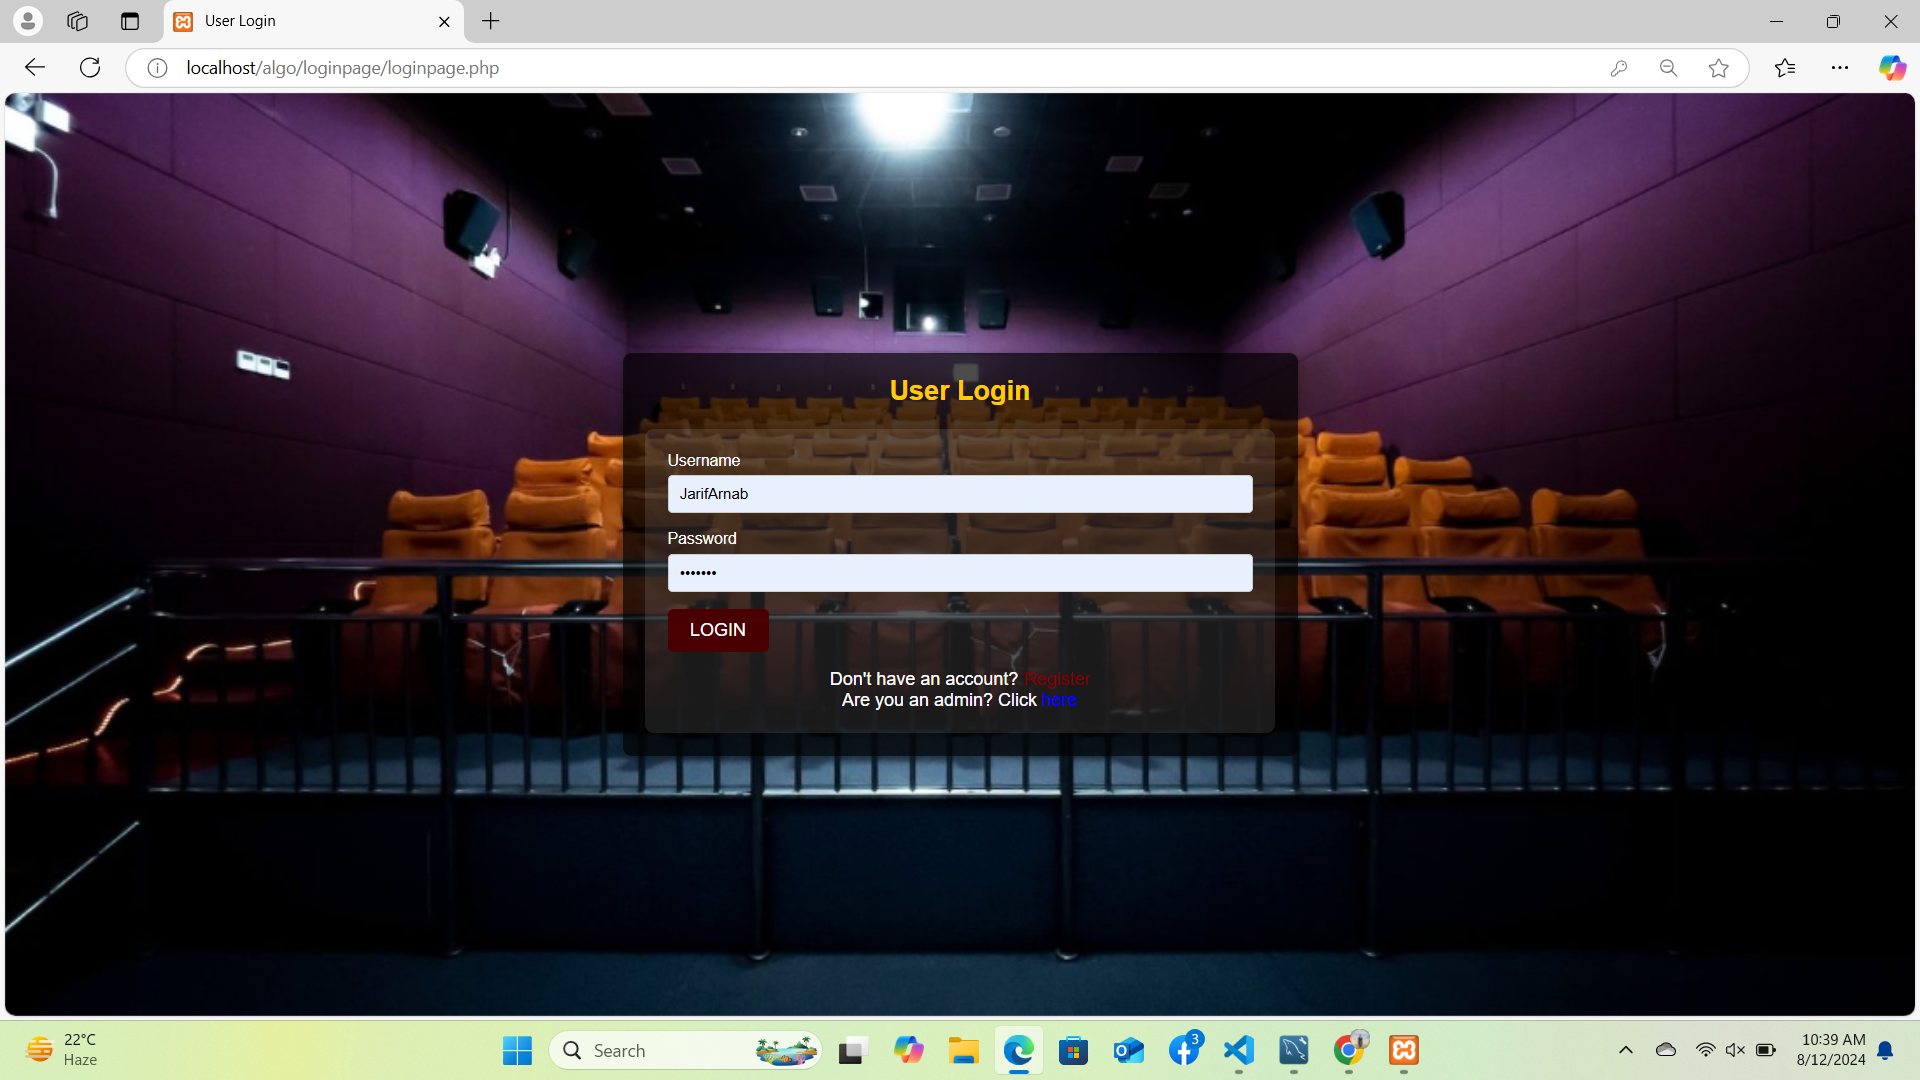
\includegraphics[width=\textwidth]{Photo01.png}
    \caption{LoginPage}
    \label{fig:photo01}
\end{figure}

\begin{figure}[h!]
    \centering
    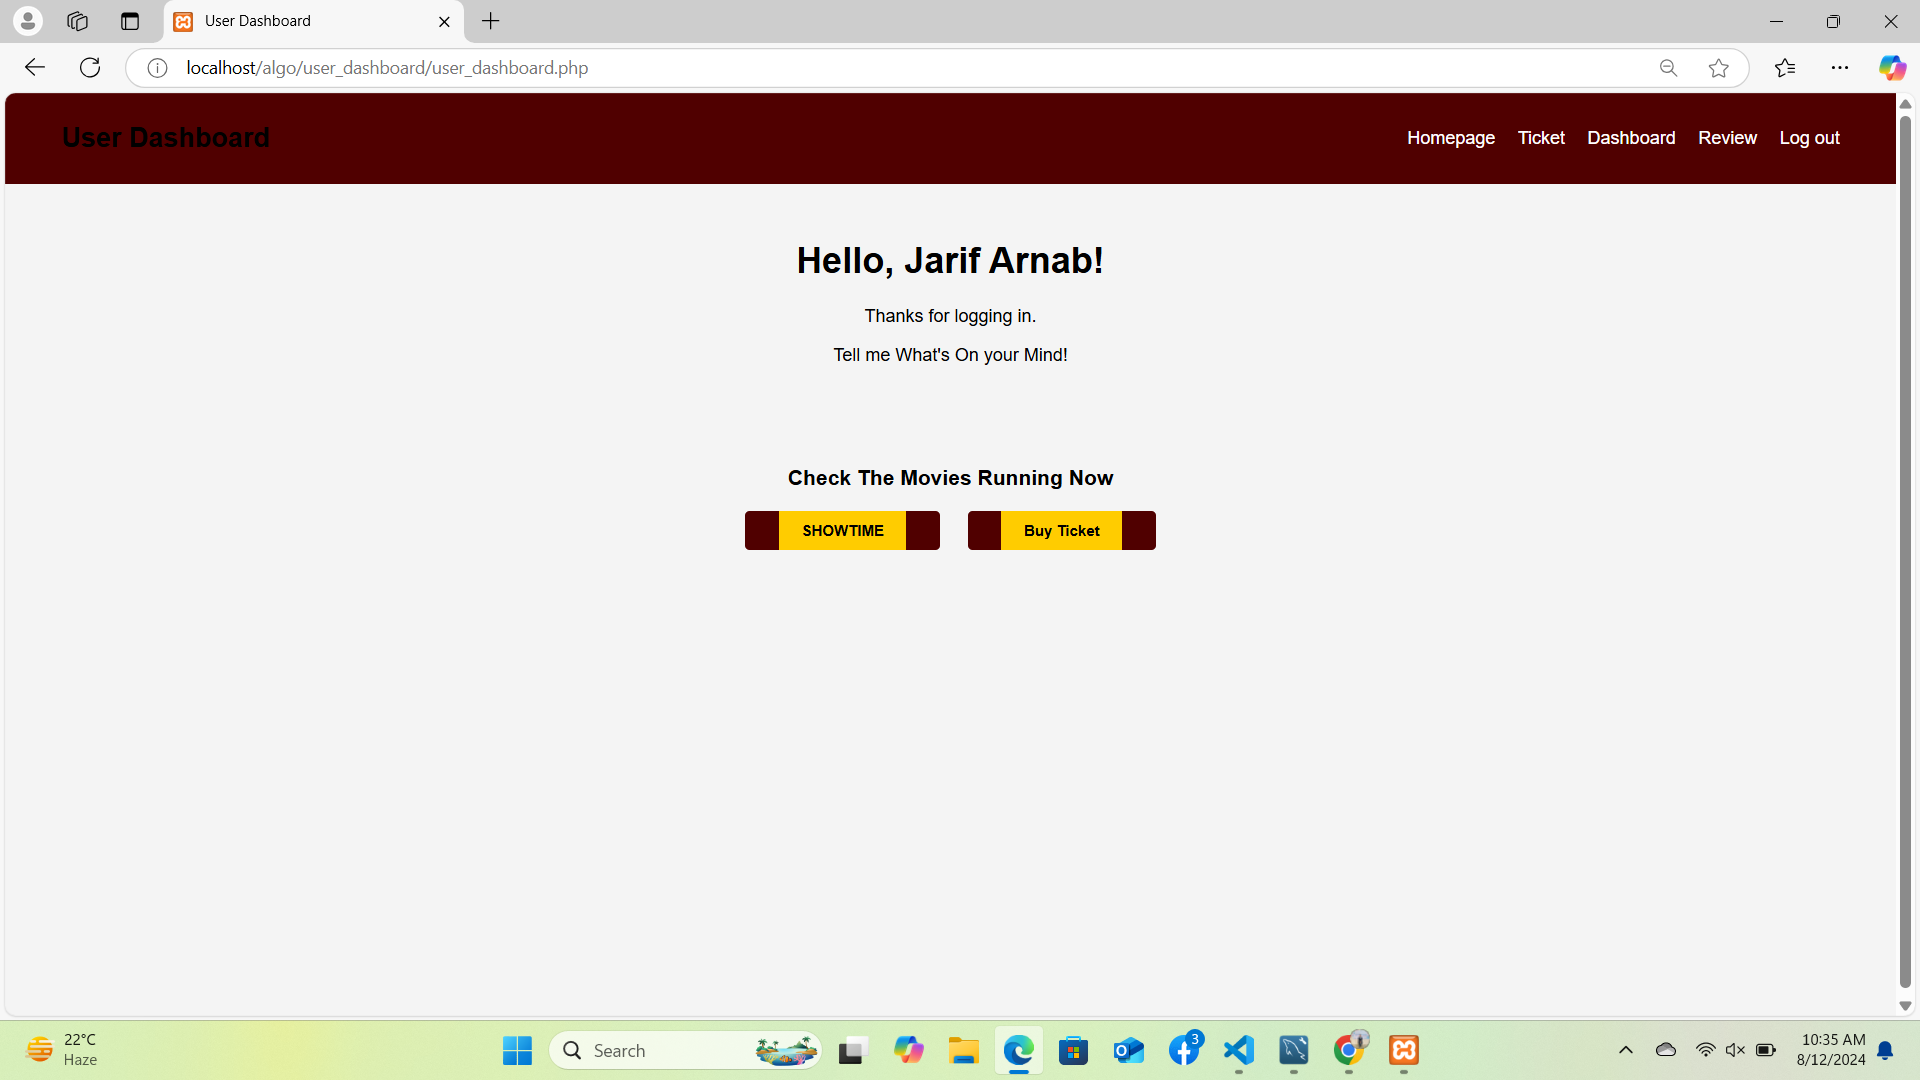
\includegraphics[width=\textwidth]{Photo2.png}
    \caption{UserDashboard}
    \label{fig:photo02}
\end{figure}
\newpage

\begin{figure}[h!]
    \centering
    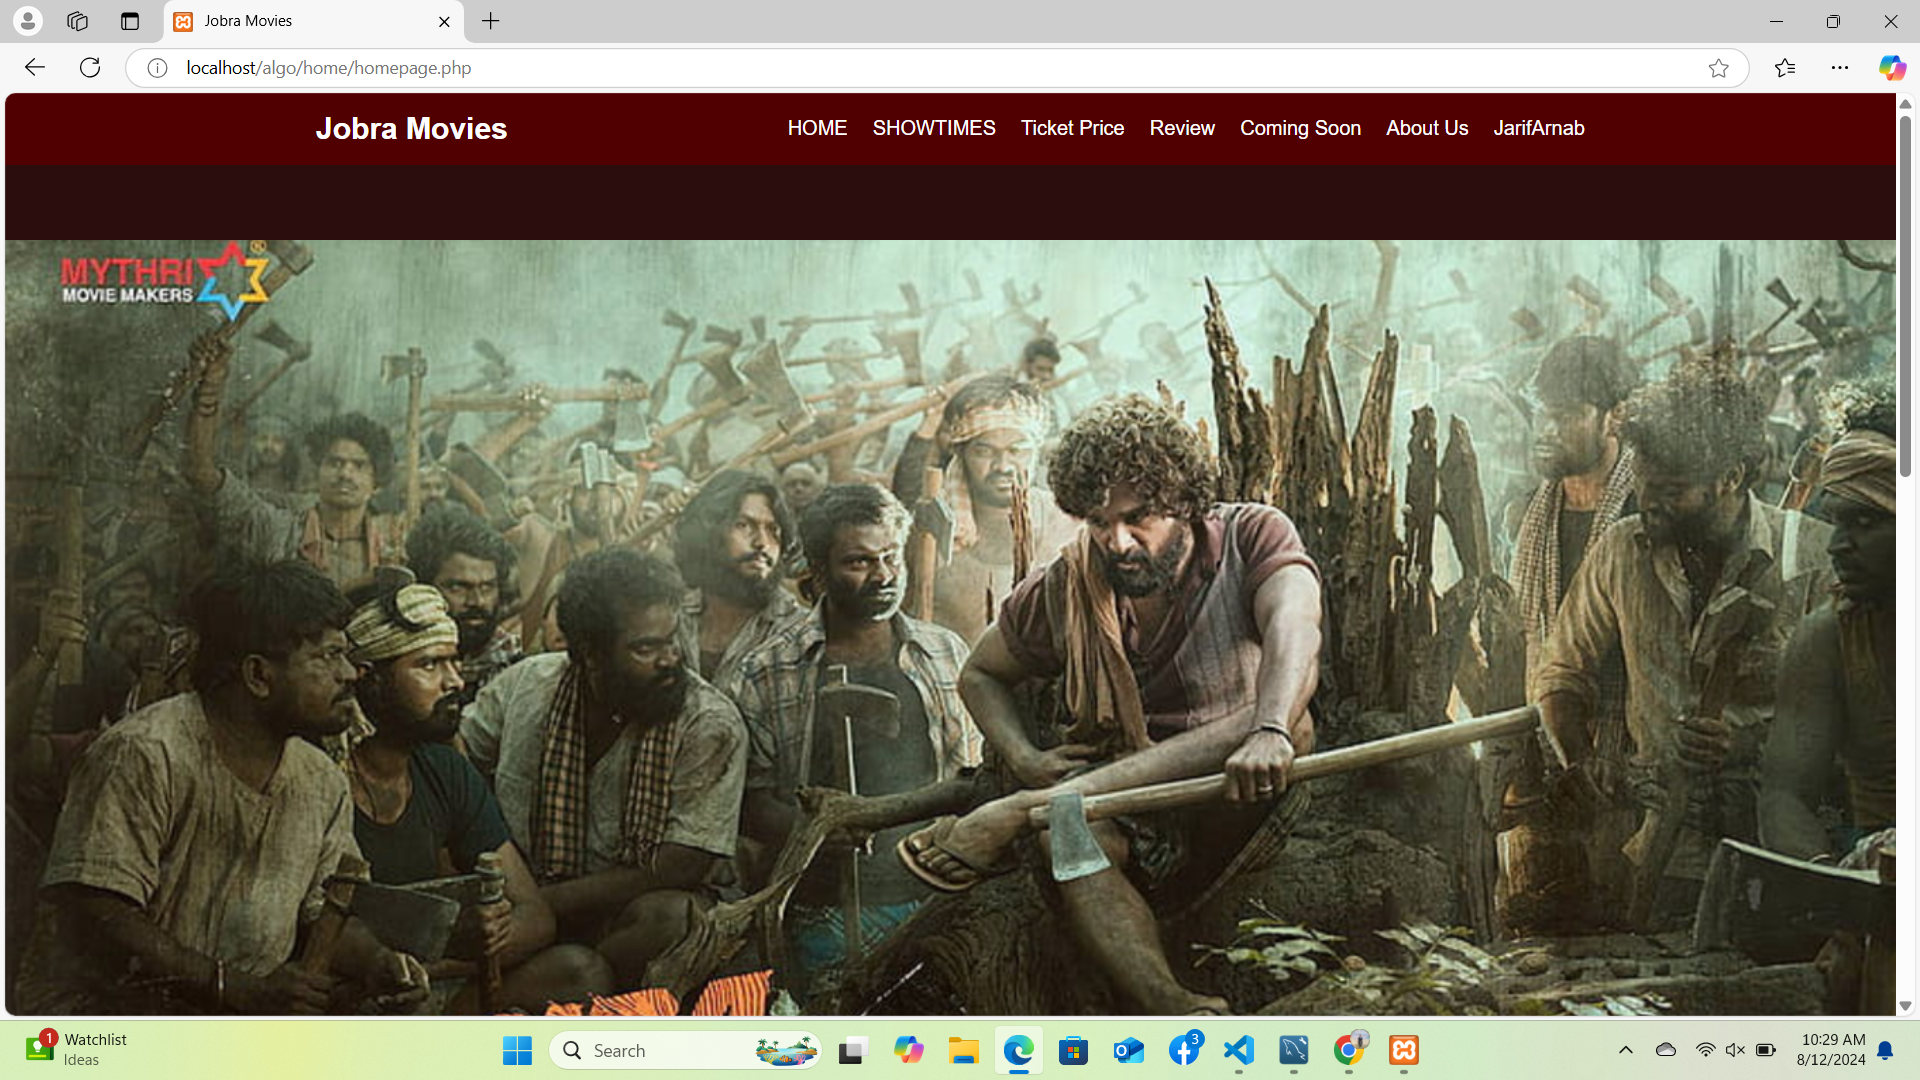
\includegraphics[width=\textwidth]{Photo02.png}
    \caption{Homepage}
    \label{fig:photo03}
\end{figure}

\begin{figure}[h!]
    \centering
    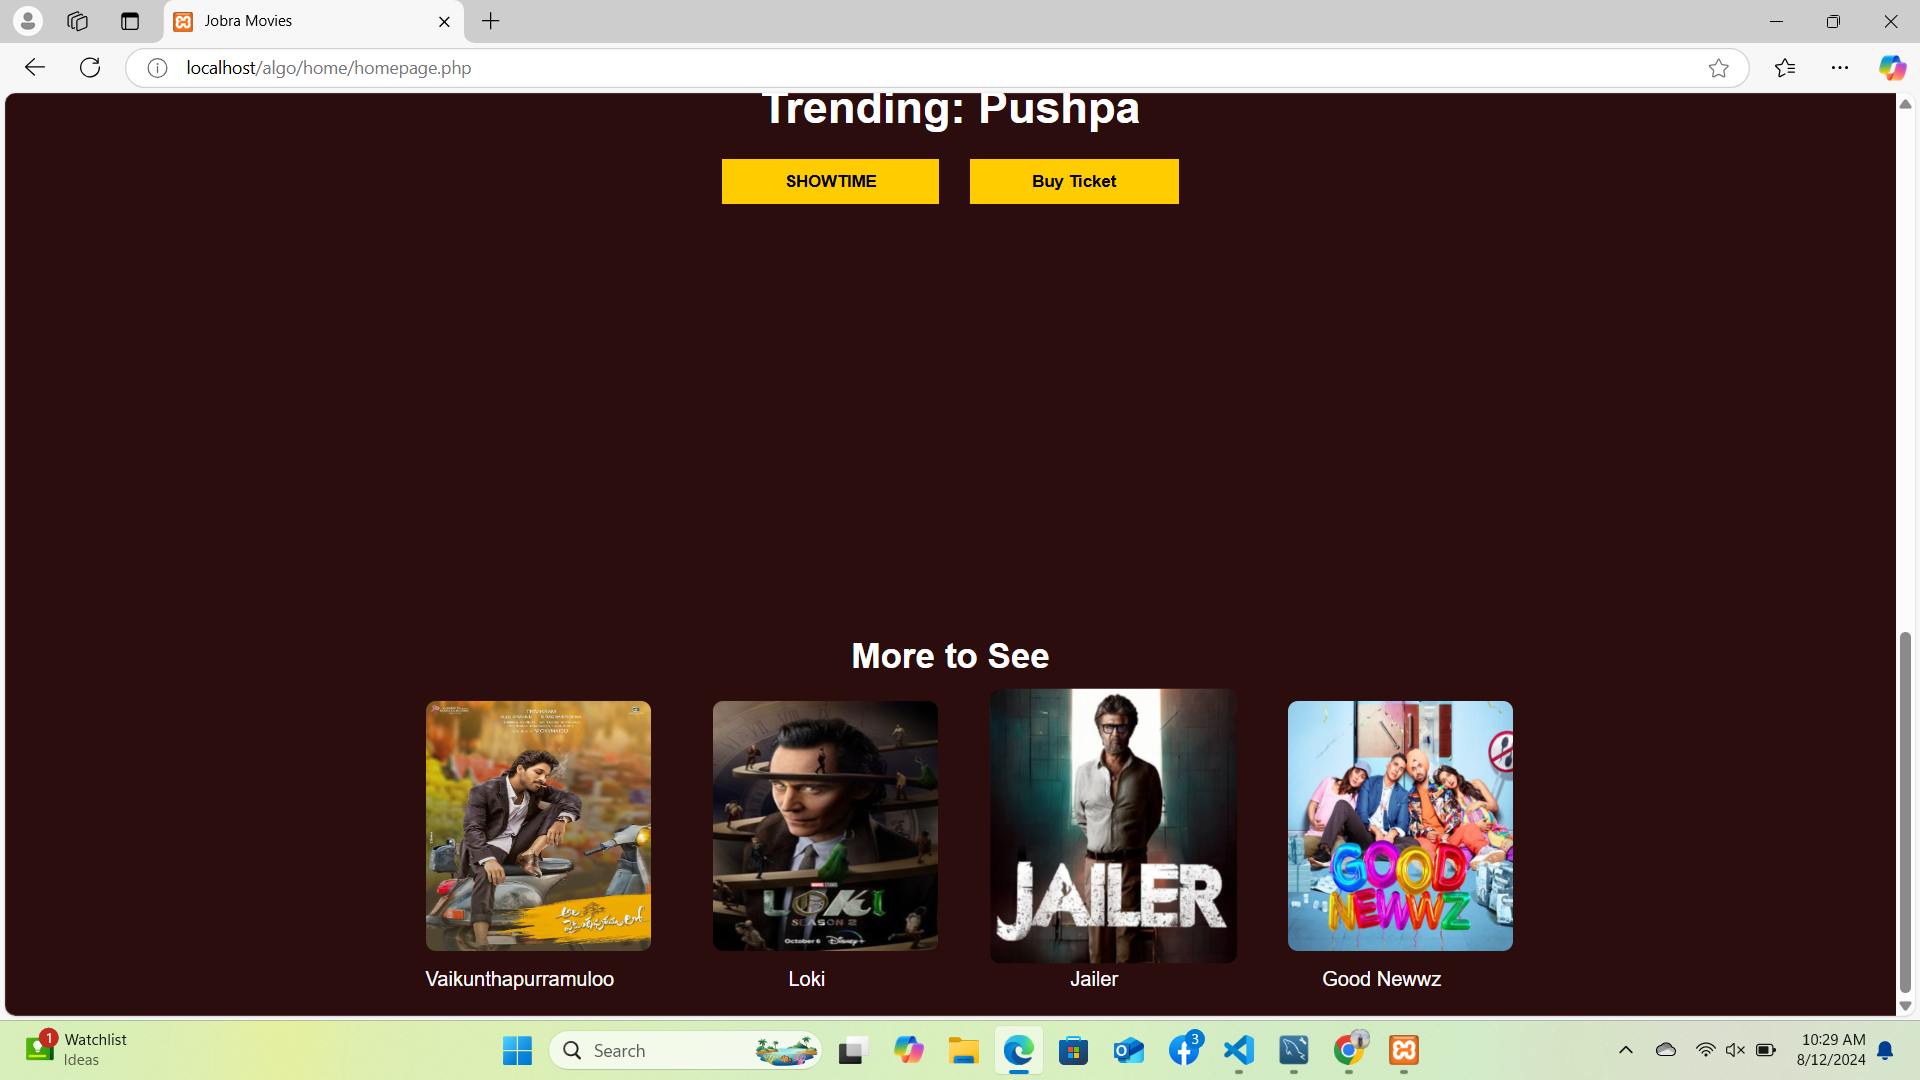
\includegraphics[width=\textwidth]{Photo03.png}
    \caption{Homepage}
    \label{fig:photo04}
\end{figure}
\newpage
\begin{figure}[h!]
    \centering
    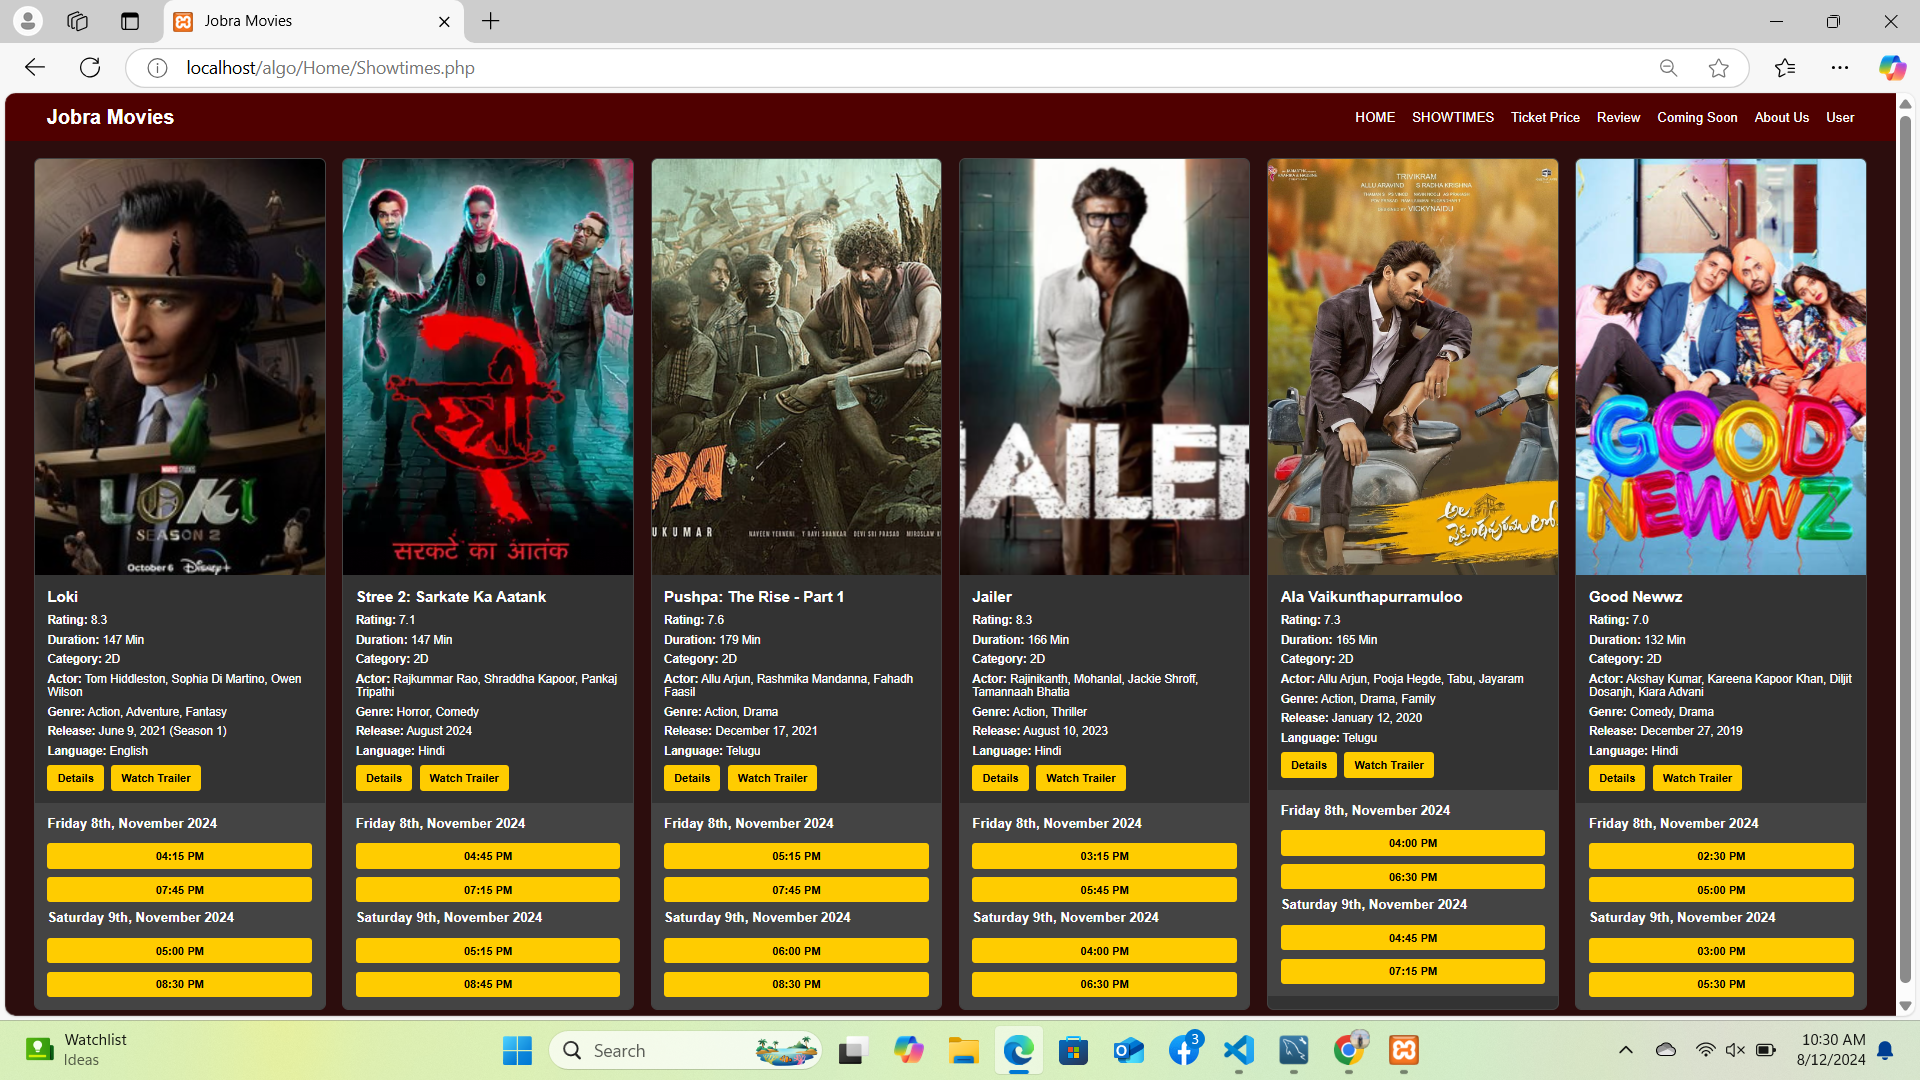
\includegraphics[width=\textwidth]{Photo04.png}
    \caption{Showtimes}
    \label{fig:photo05}
\end{figure}

\begin{figure}[h!]
    \centering
    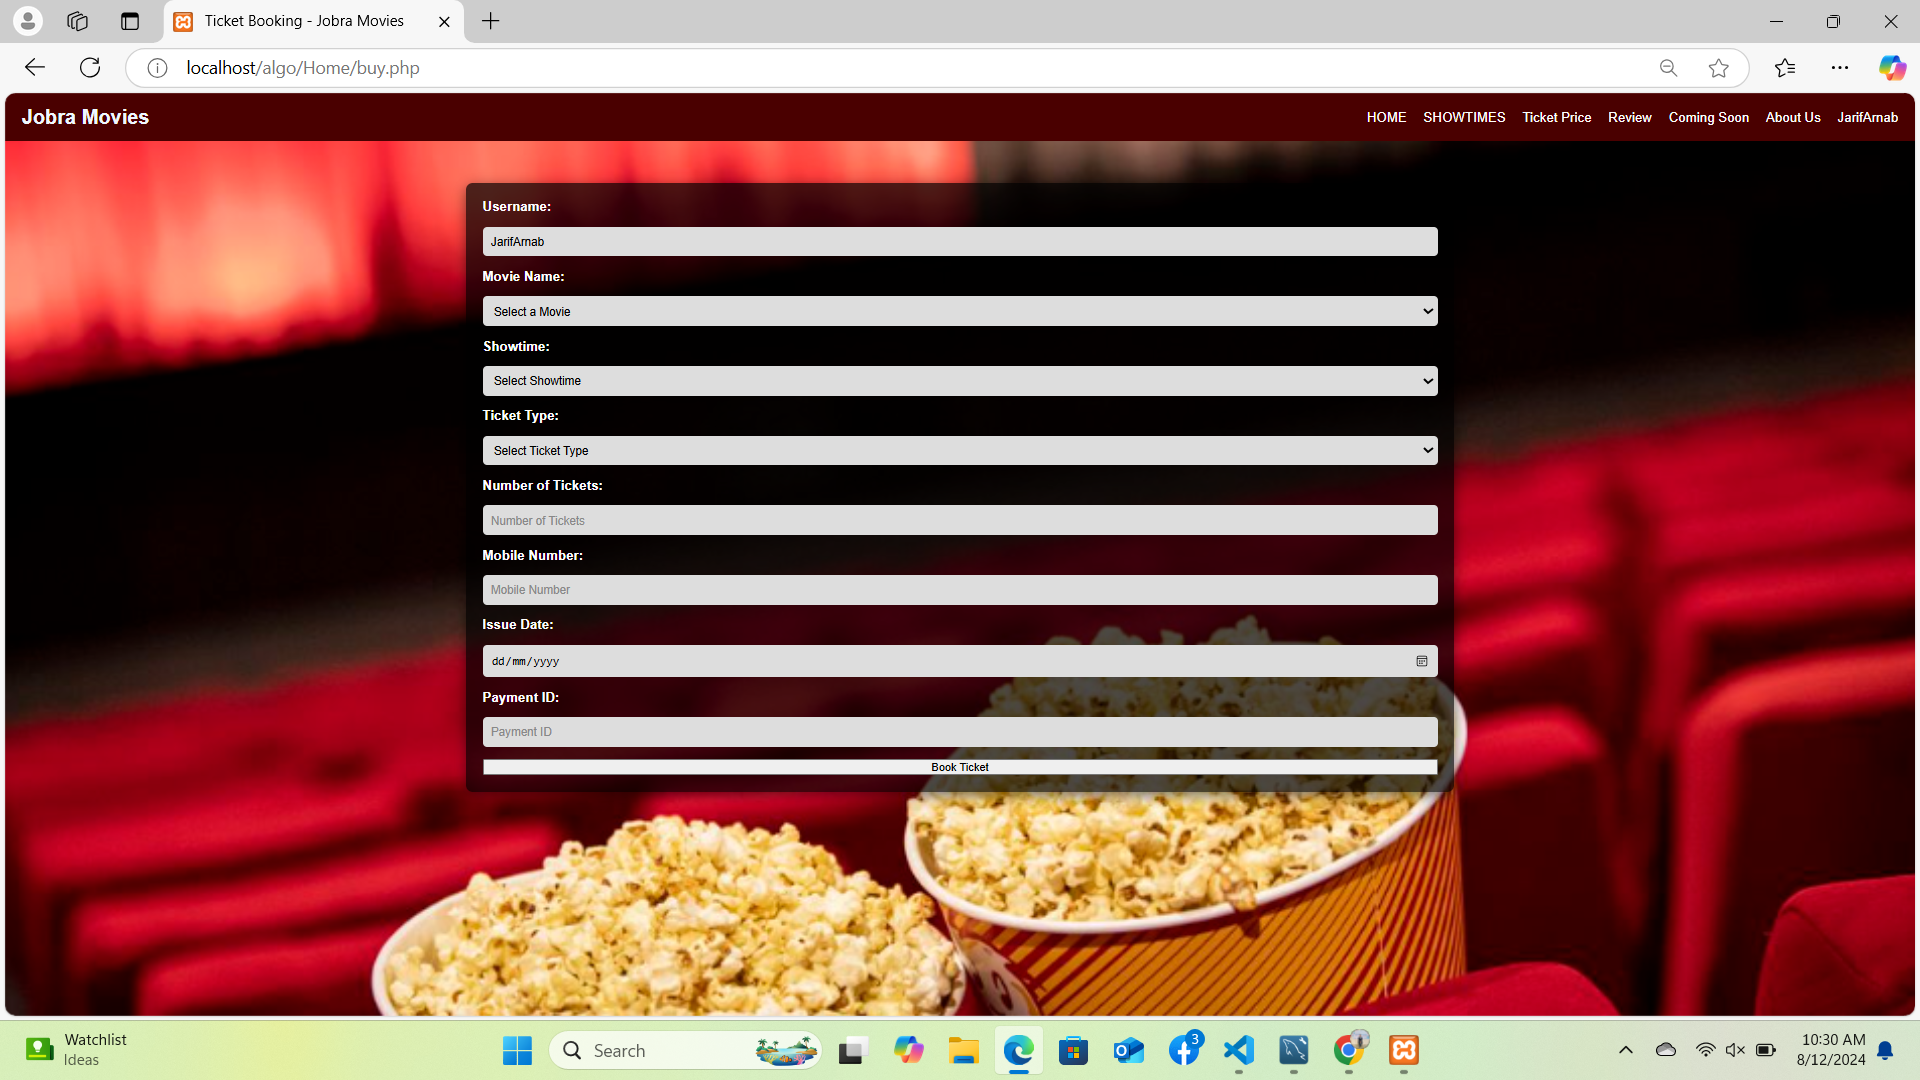
\includegraphics[width=\textwidth]{Photo05.png}
    \caption{Buy Tickets}
    \label{fig:photo06}
\end{figure}
\newpage





\begin{figure}[h!]
    \centering
    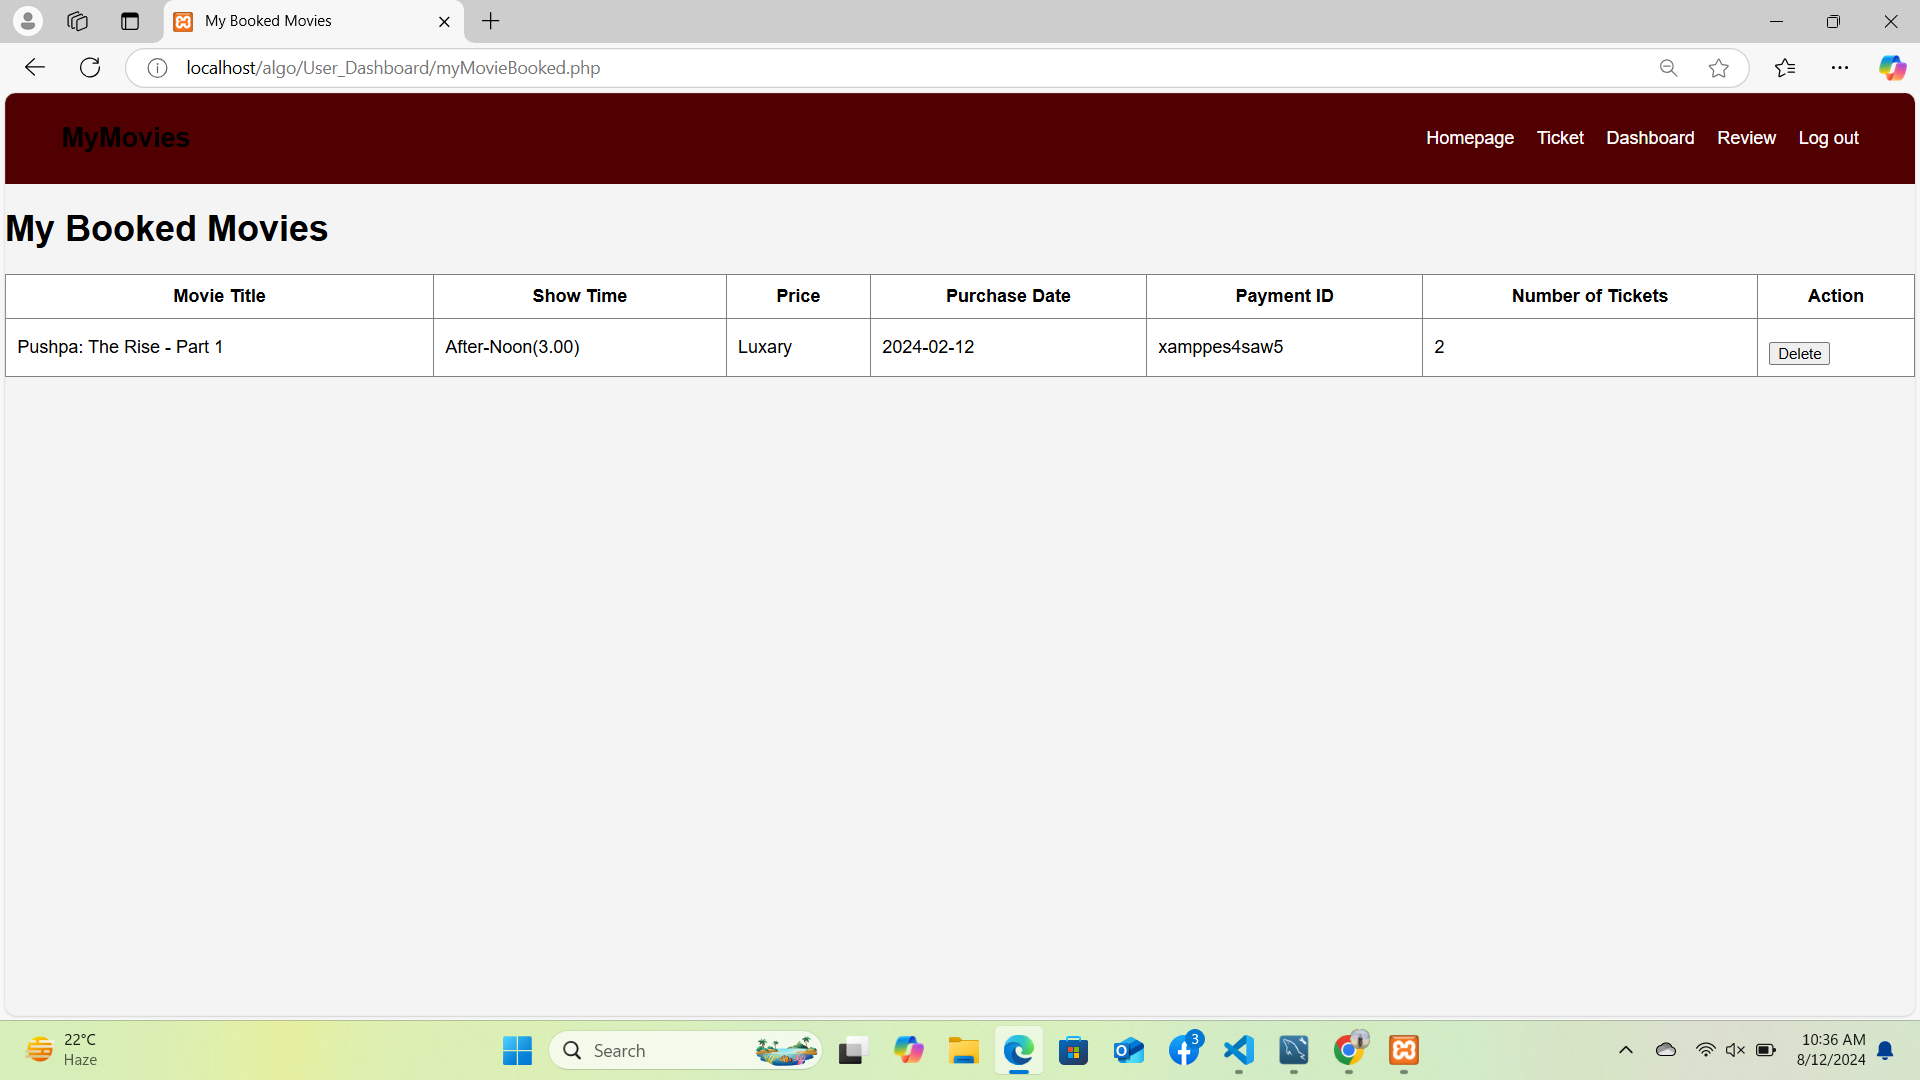
\includegraphics[width=\textwidth]{Photo5.png}
    \caption{Booked Movies list by user}
    \label{fig:photo07}
\end{figure}

\begin{figure}[h!]
    \centering
    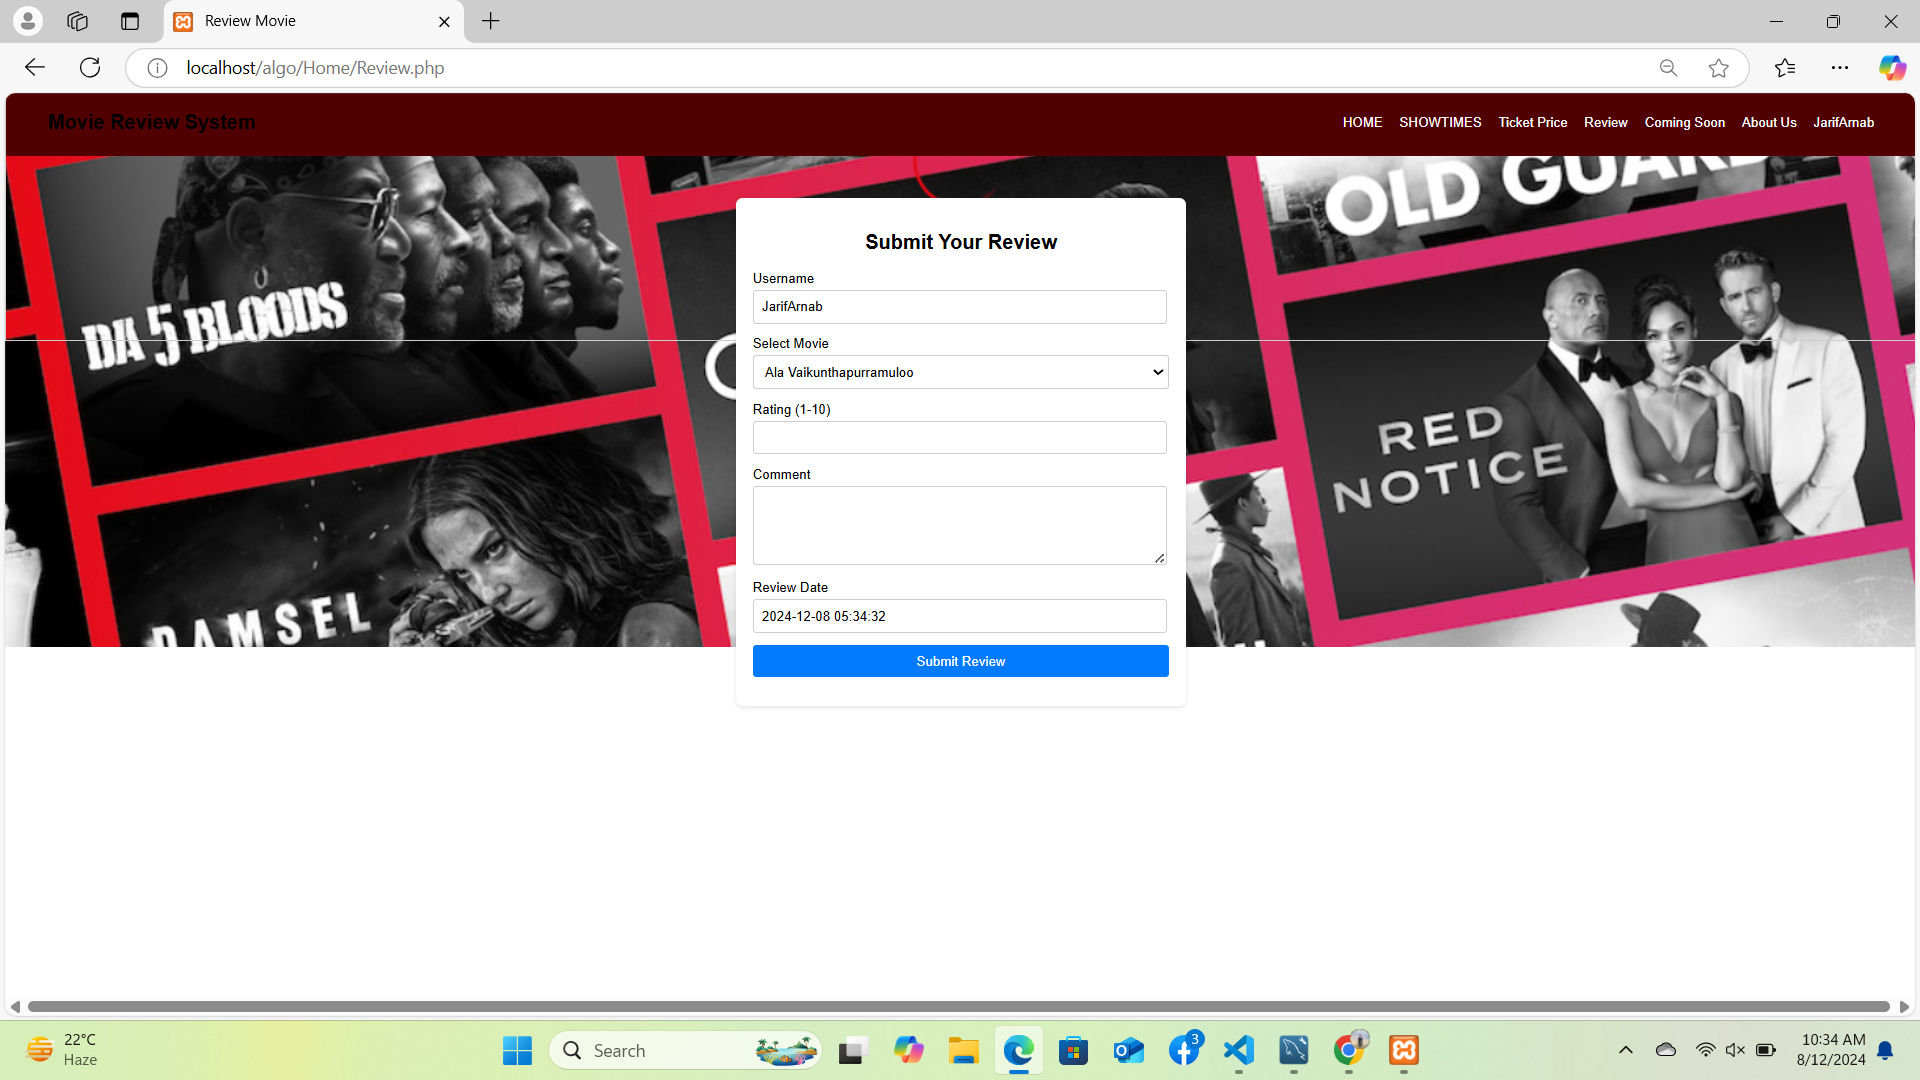
\includegraphics[width=\textwidth]{Photo06.png}
    \caption{ReviewPage}
    \label{fig:photo08}
\end{figure}
\newpage
\begin{figure}[h!]
    \centering
    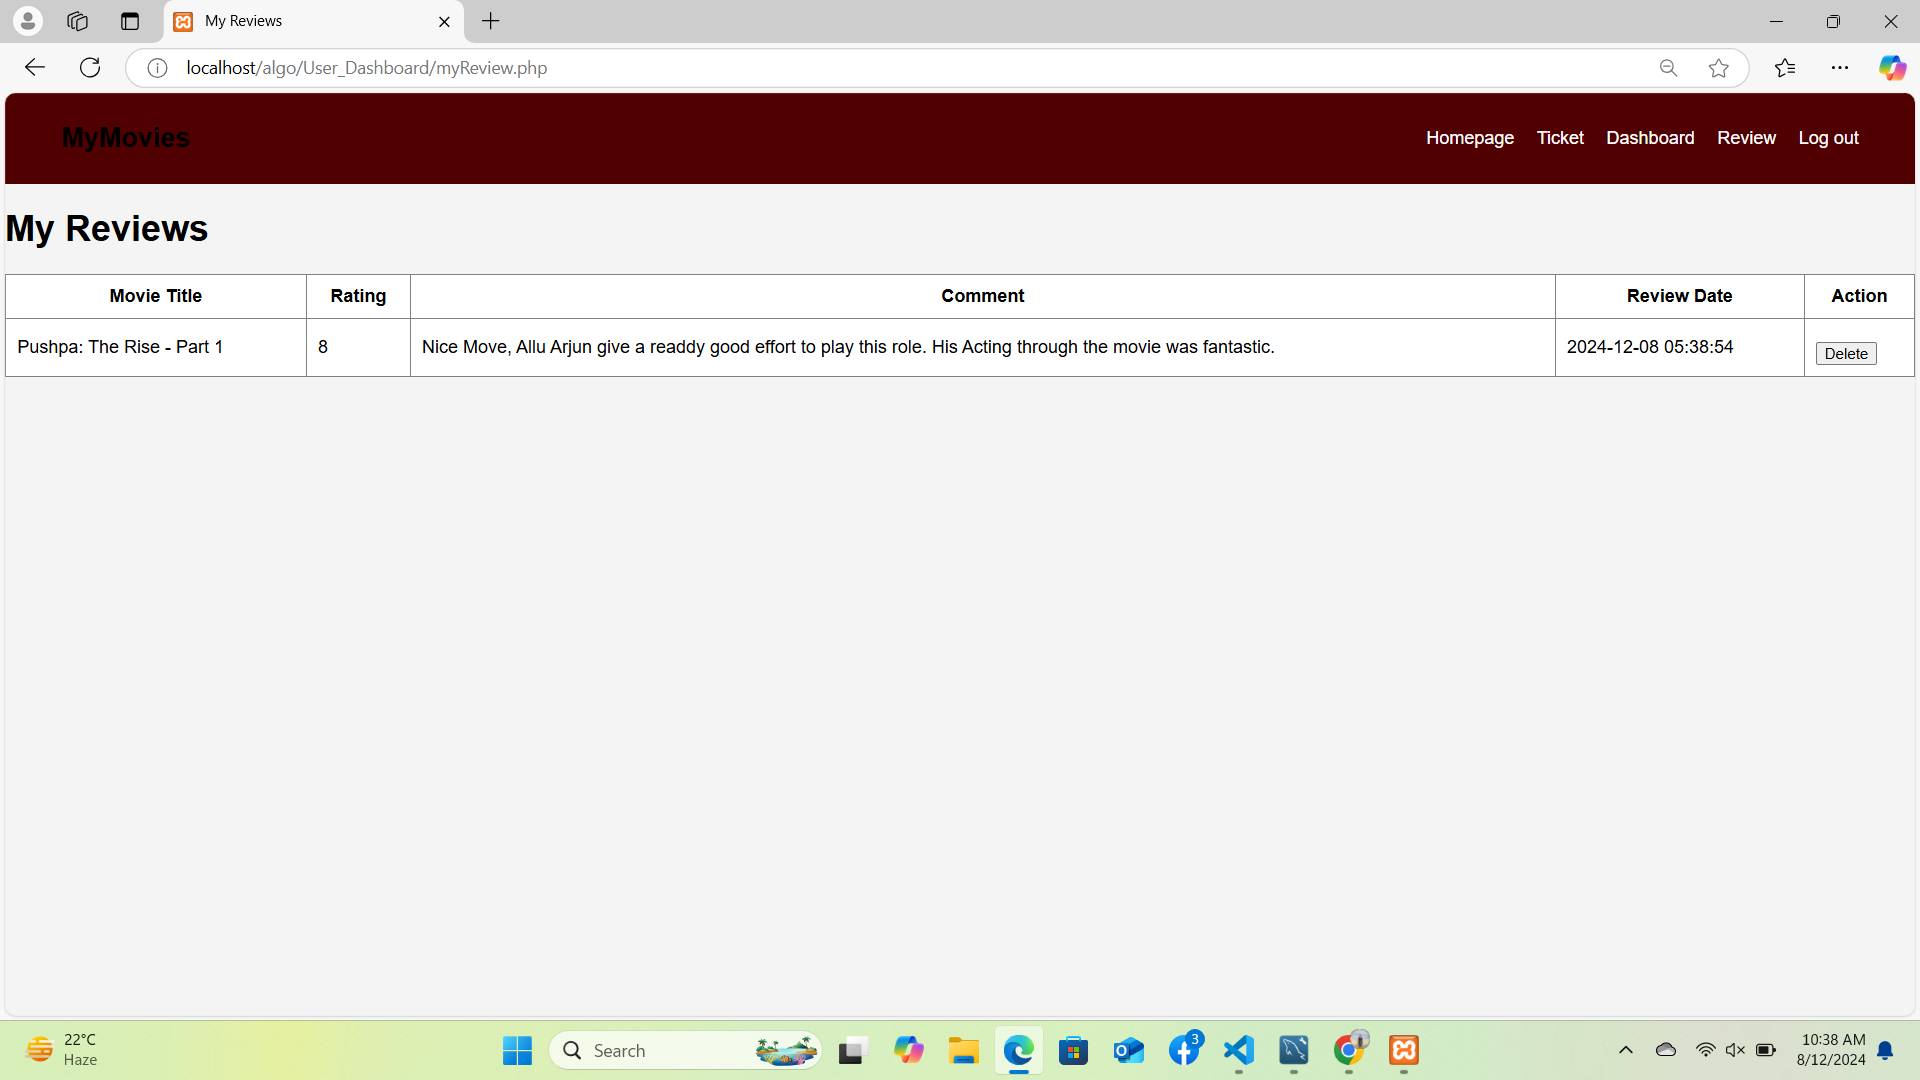
\includegraphics[width=\textwidth]{Photo6.png}
    \caption{Reviews Given by the user}
    \label{fig:photo09}
\end{figure}

\begin{figure}[h!]
    \centering
    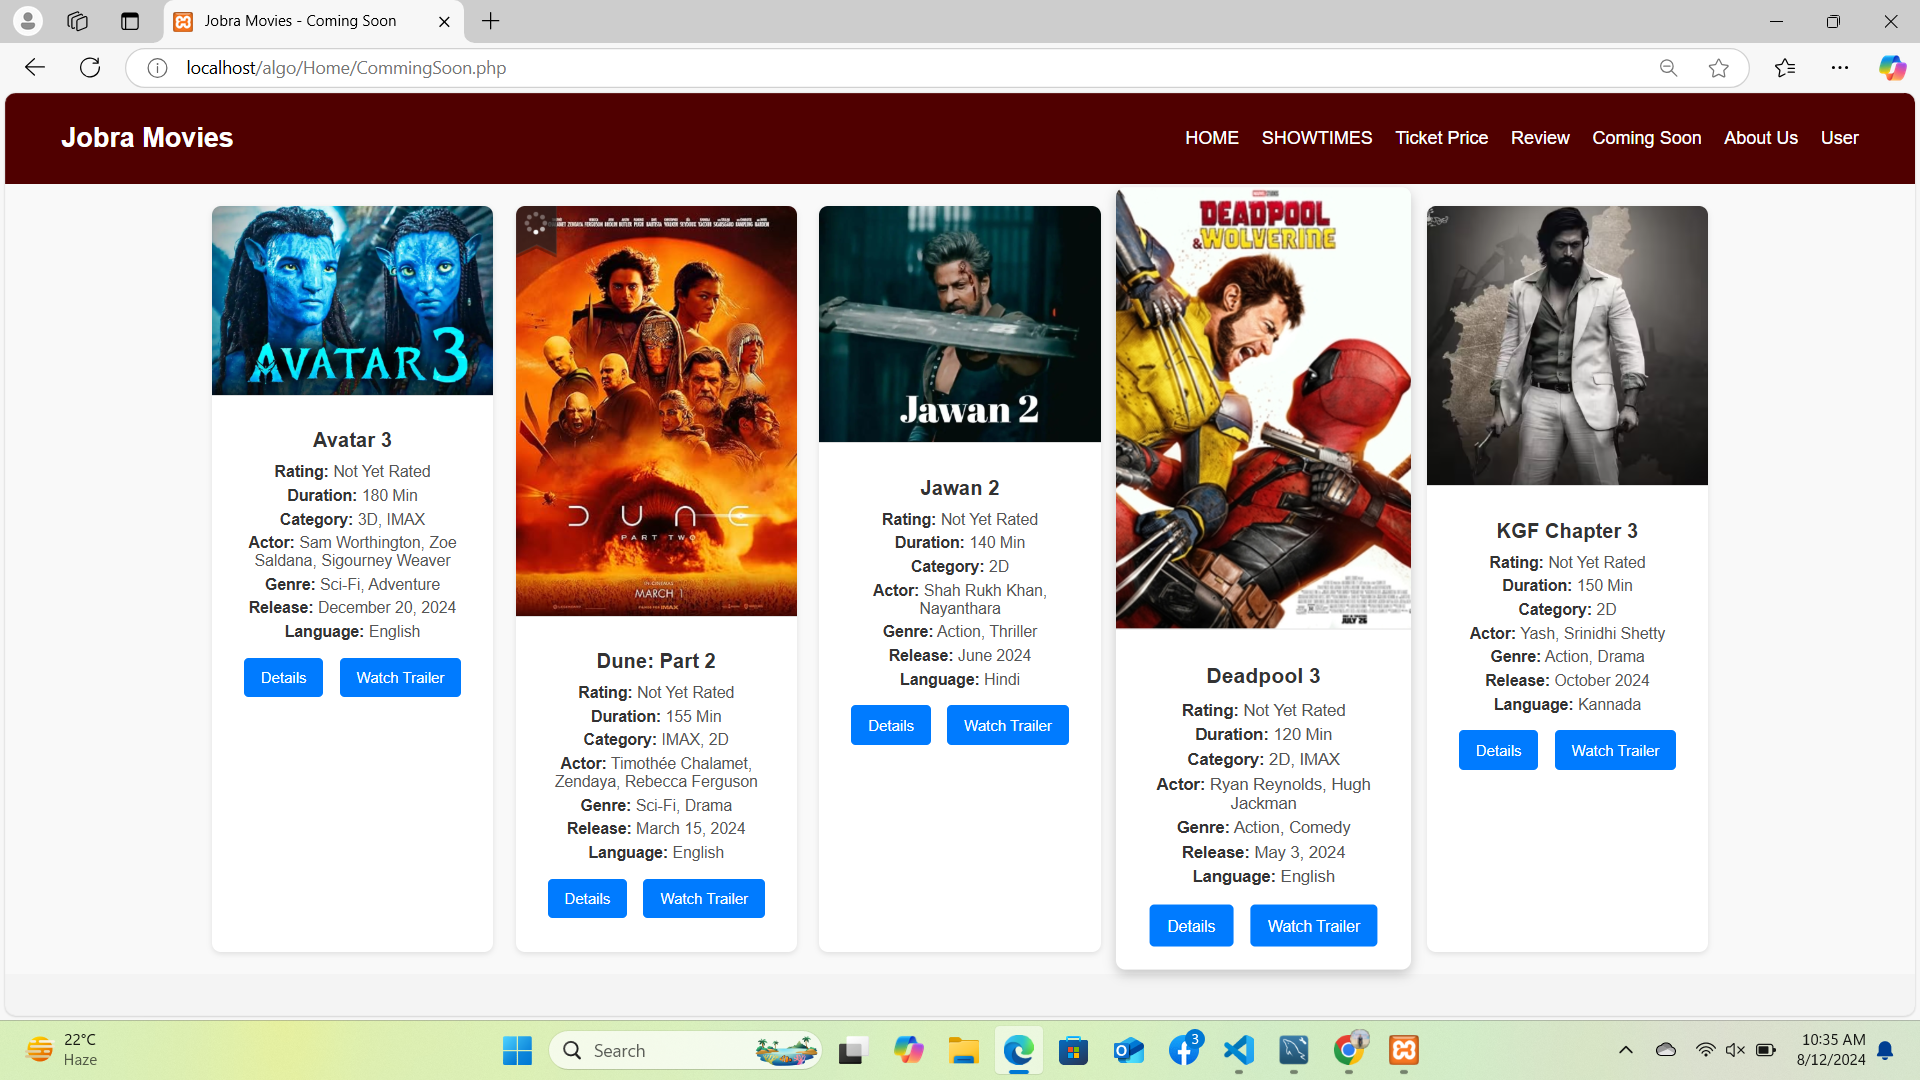
\includegraphics[width=\textwidth]{Photo07.png}
    \caption{Comming Soon}
    \label{fig:photo10}
\end{figure}
\newpage
\begin{figure}[h!]
    \centering
    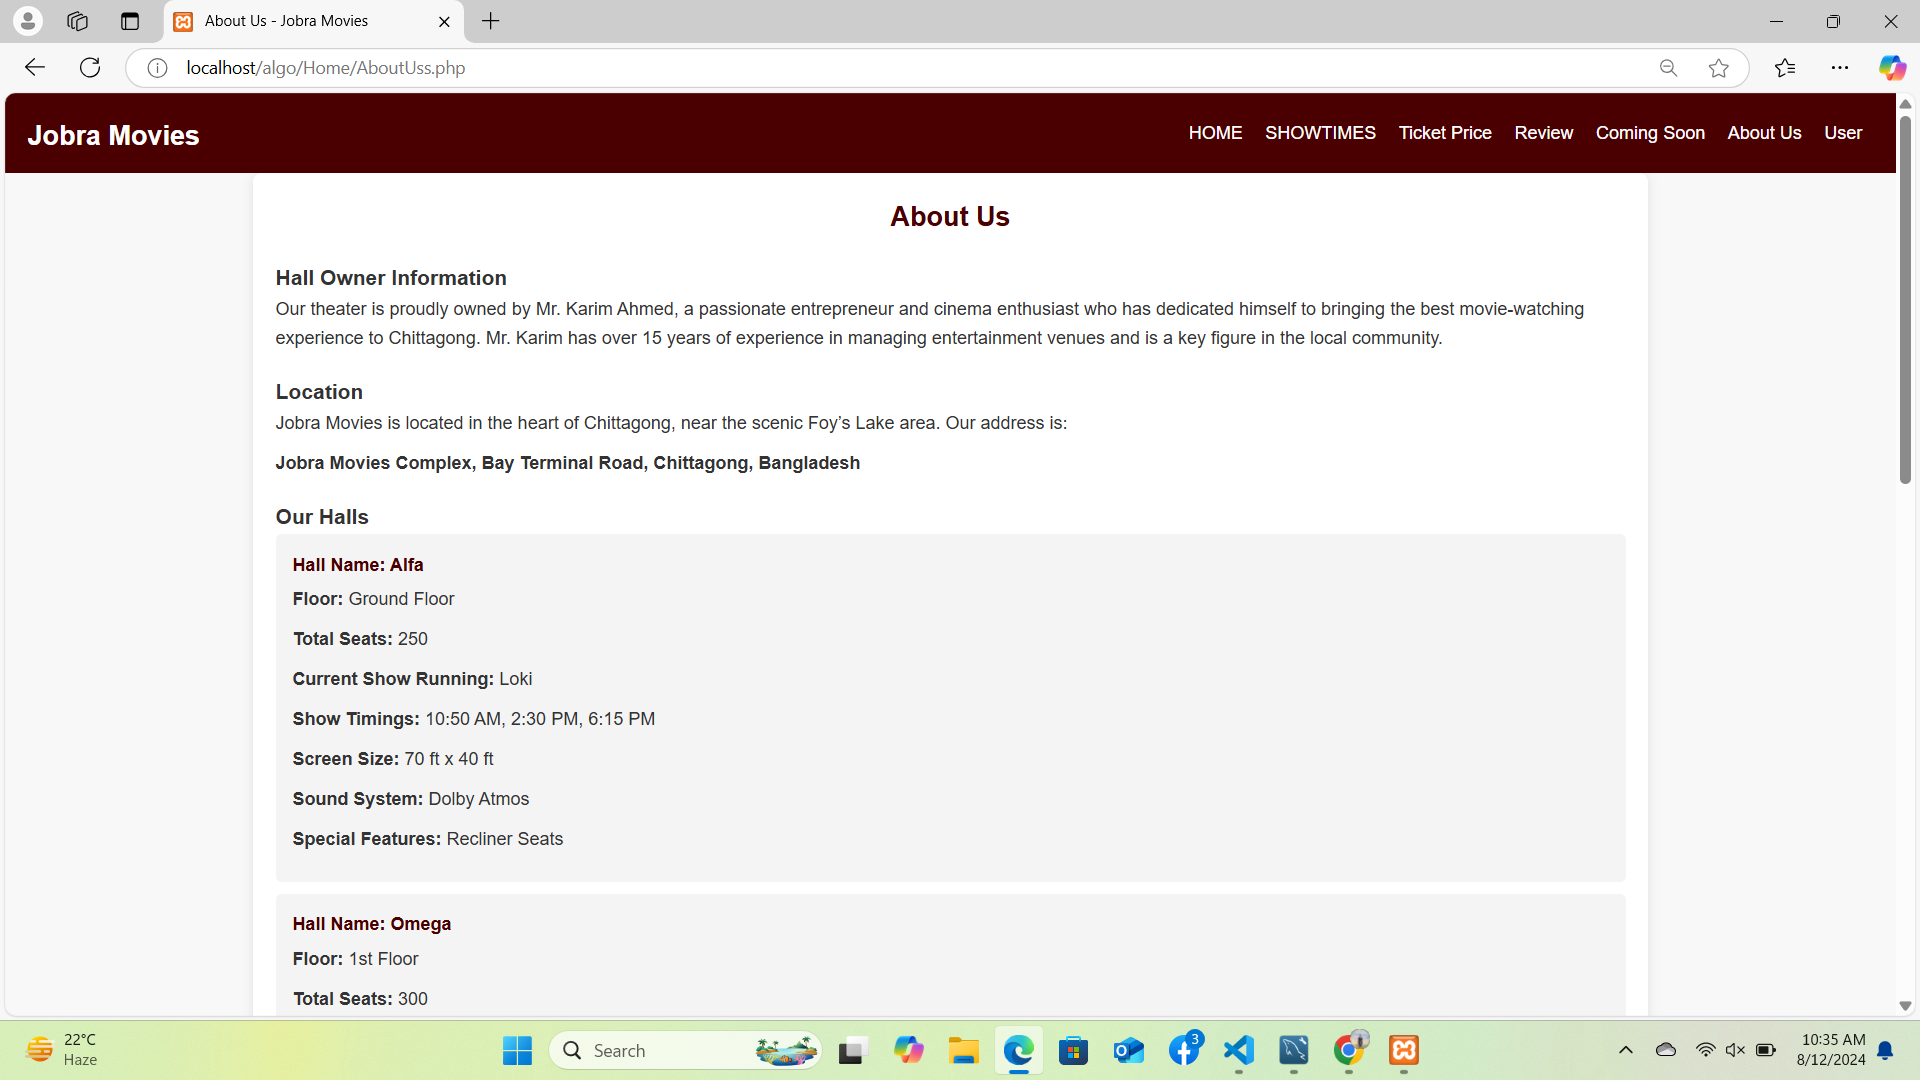
\includegraphics[width=\textwidth]{Photo08.png}
    \caption{About Maker}
    \label{fig:photo11}
\end{figure}

\begin{figure}[h!]
    \centering
    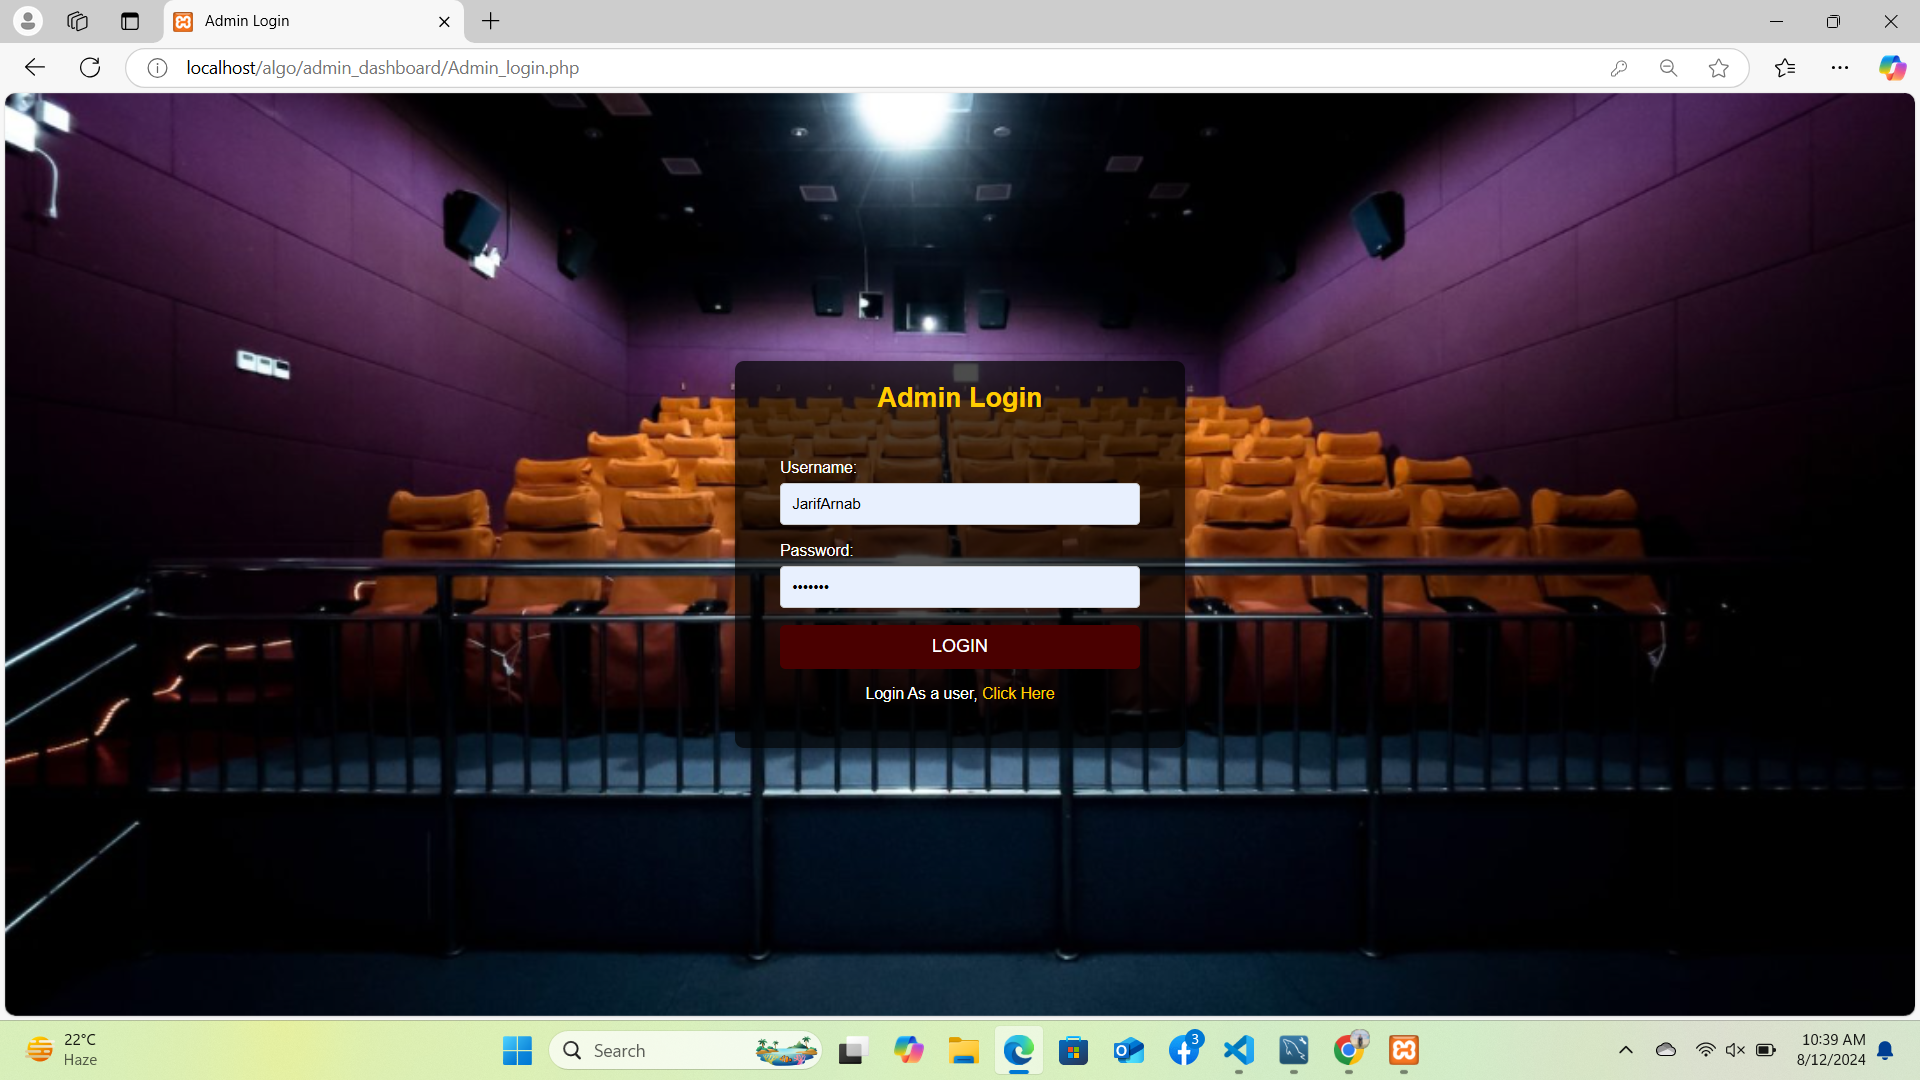
\includegraphics[width=\textwidth]{Photo09.png}
    \caption{Admin Login}
    \label{fig:photo12}
\end{figure}

\newpage



\begin{figure}[h!]
    \centering
    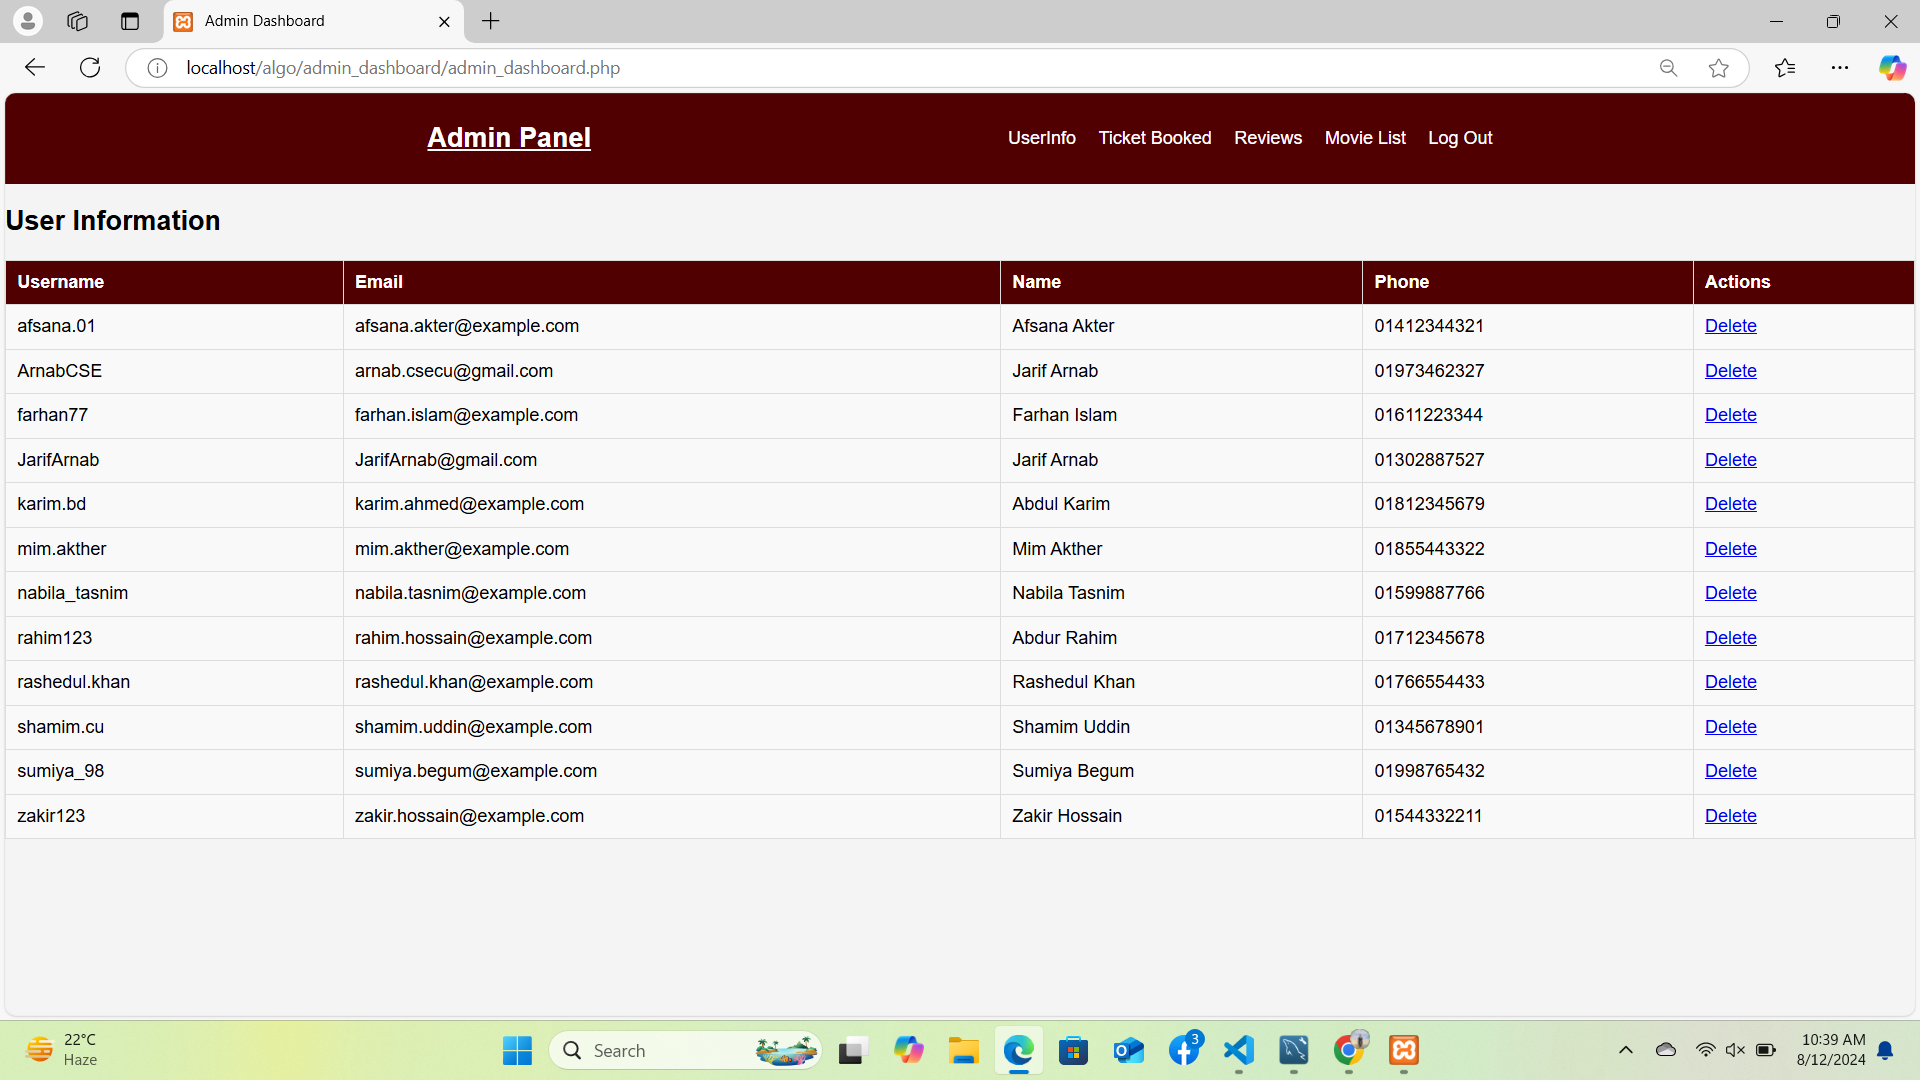
\includegraphics[width=\textwidth]{Photo10.png}
    \caption{User List}
    \label{fig:photo13}
\end{figure}

\begin{figure}[h!]
    \centering
    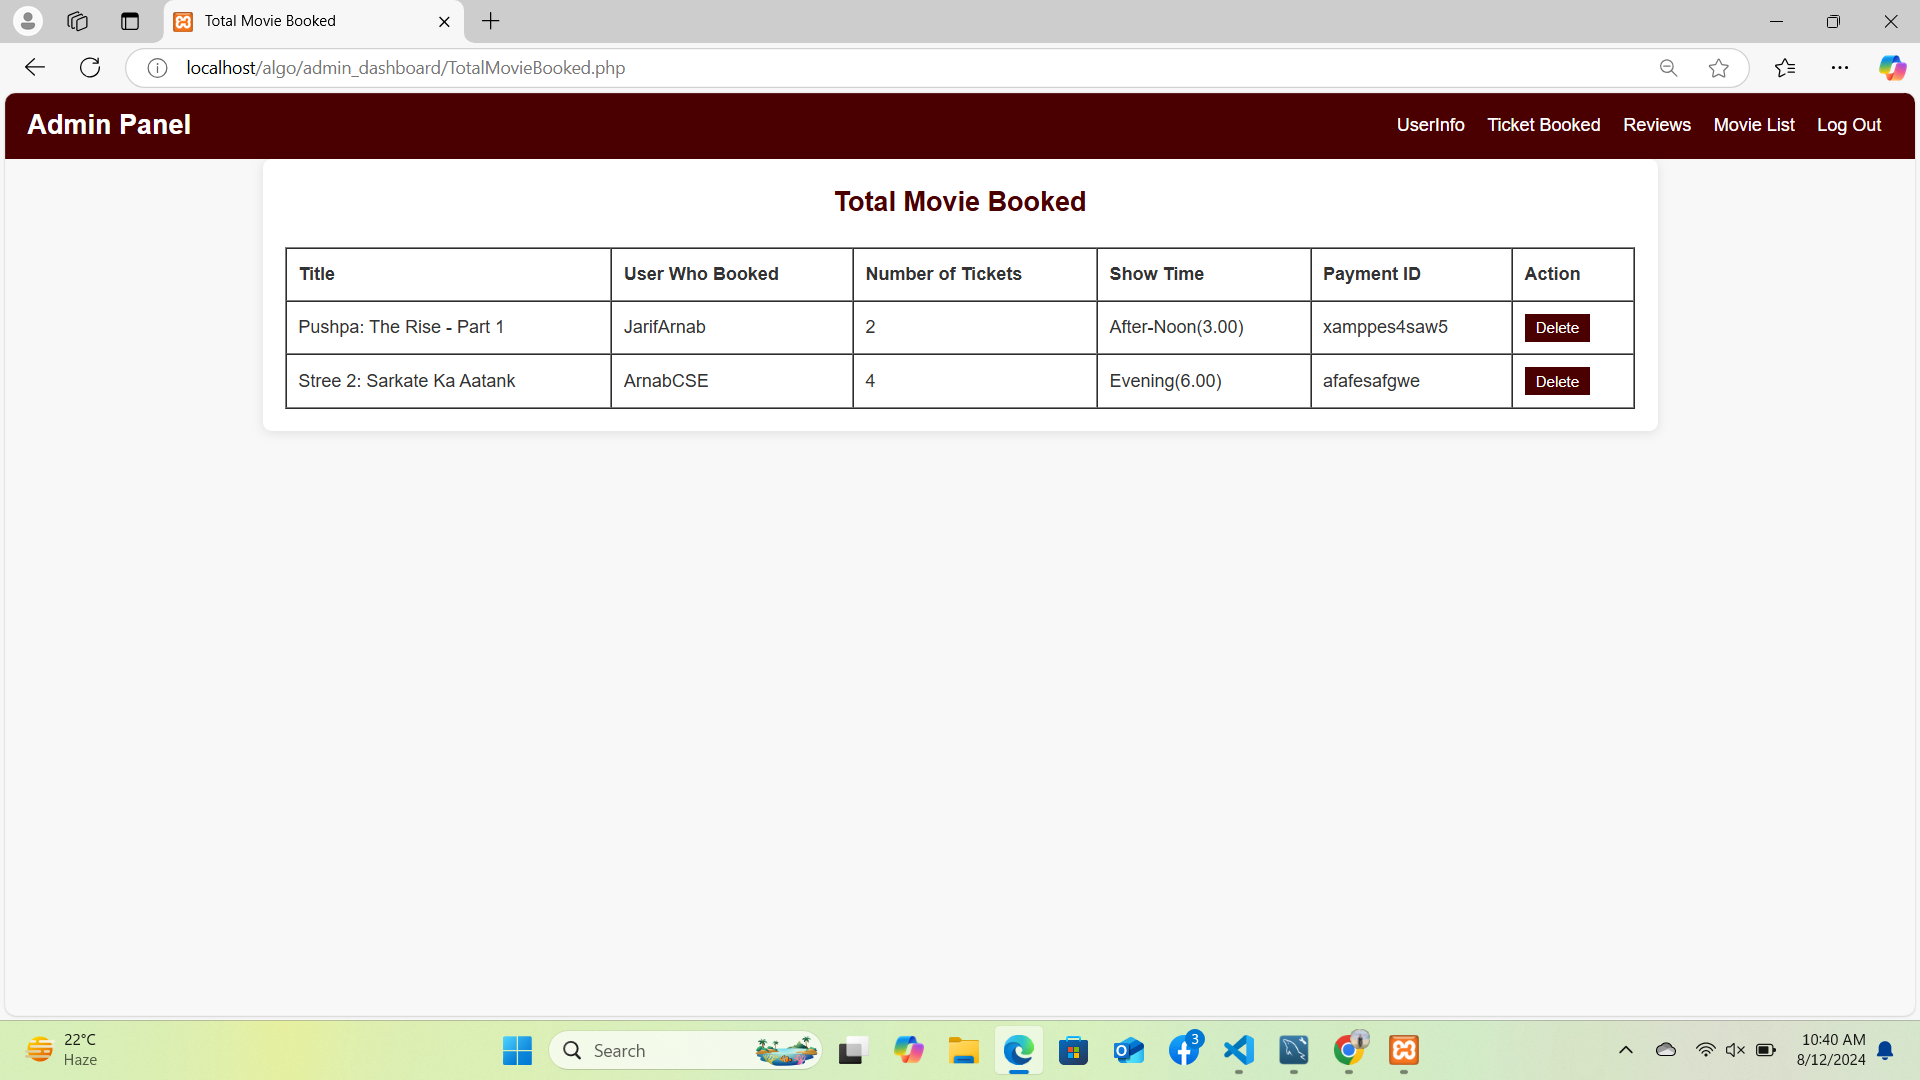
\includegraphics[width=\textwidth]{Photo11.png}
    \caption{Total Movie Booked}
    \label{fig:photo14}
\end{figure}
\newpage
\begin{figure}[h!]
    \centering
    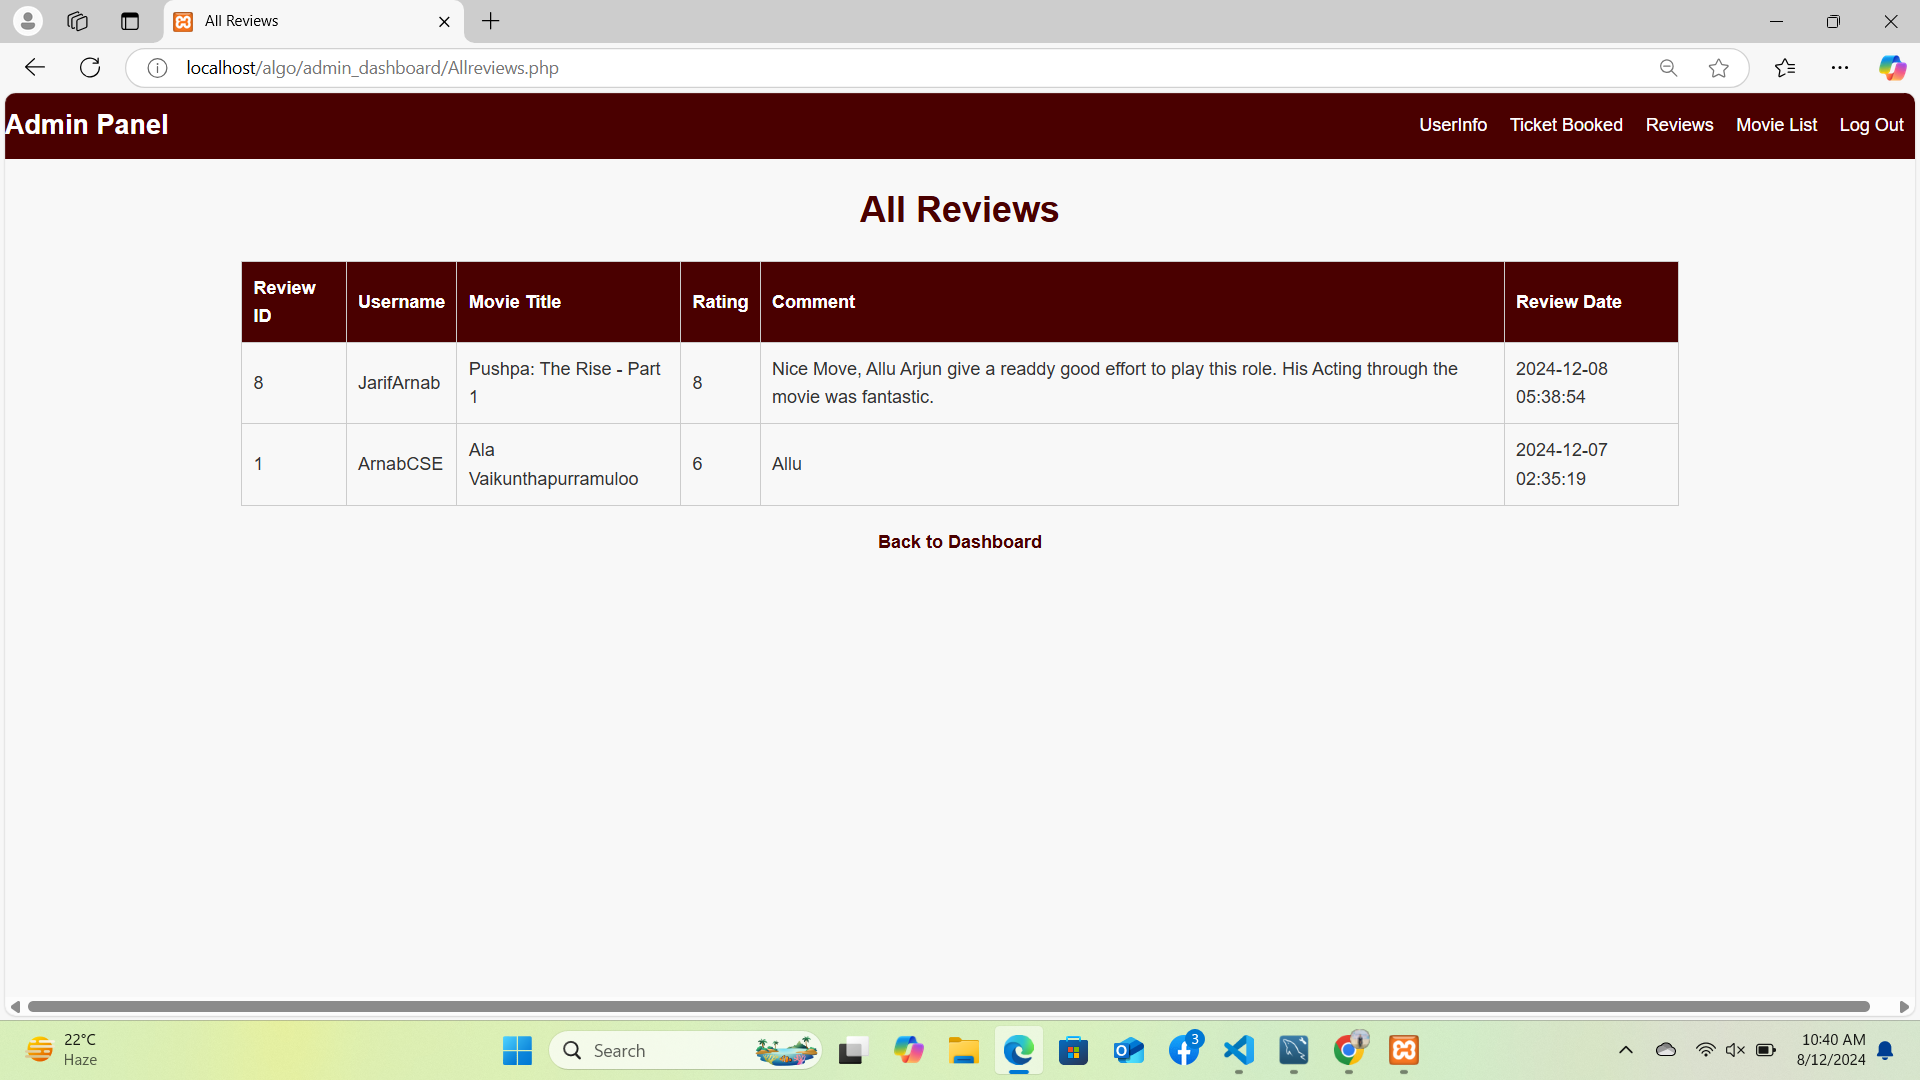
\includegraphics[width=\textwidth]{Photo12.png}
    \caption{All Reviews}
    \label{fig:photo06}
\end{figure}





\begin{figure}[h!]
    \centering
    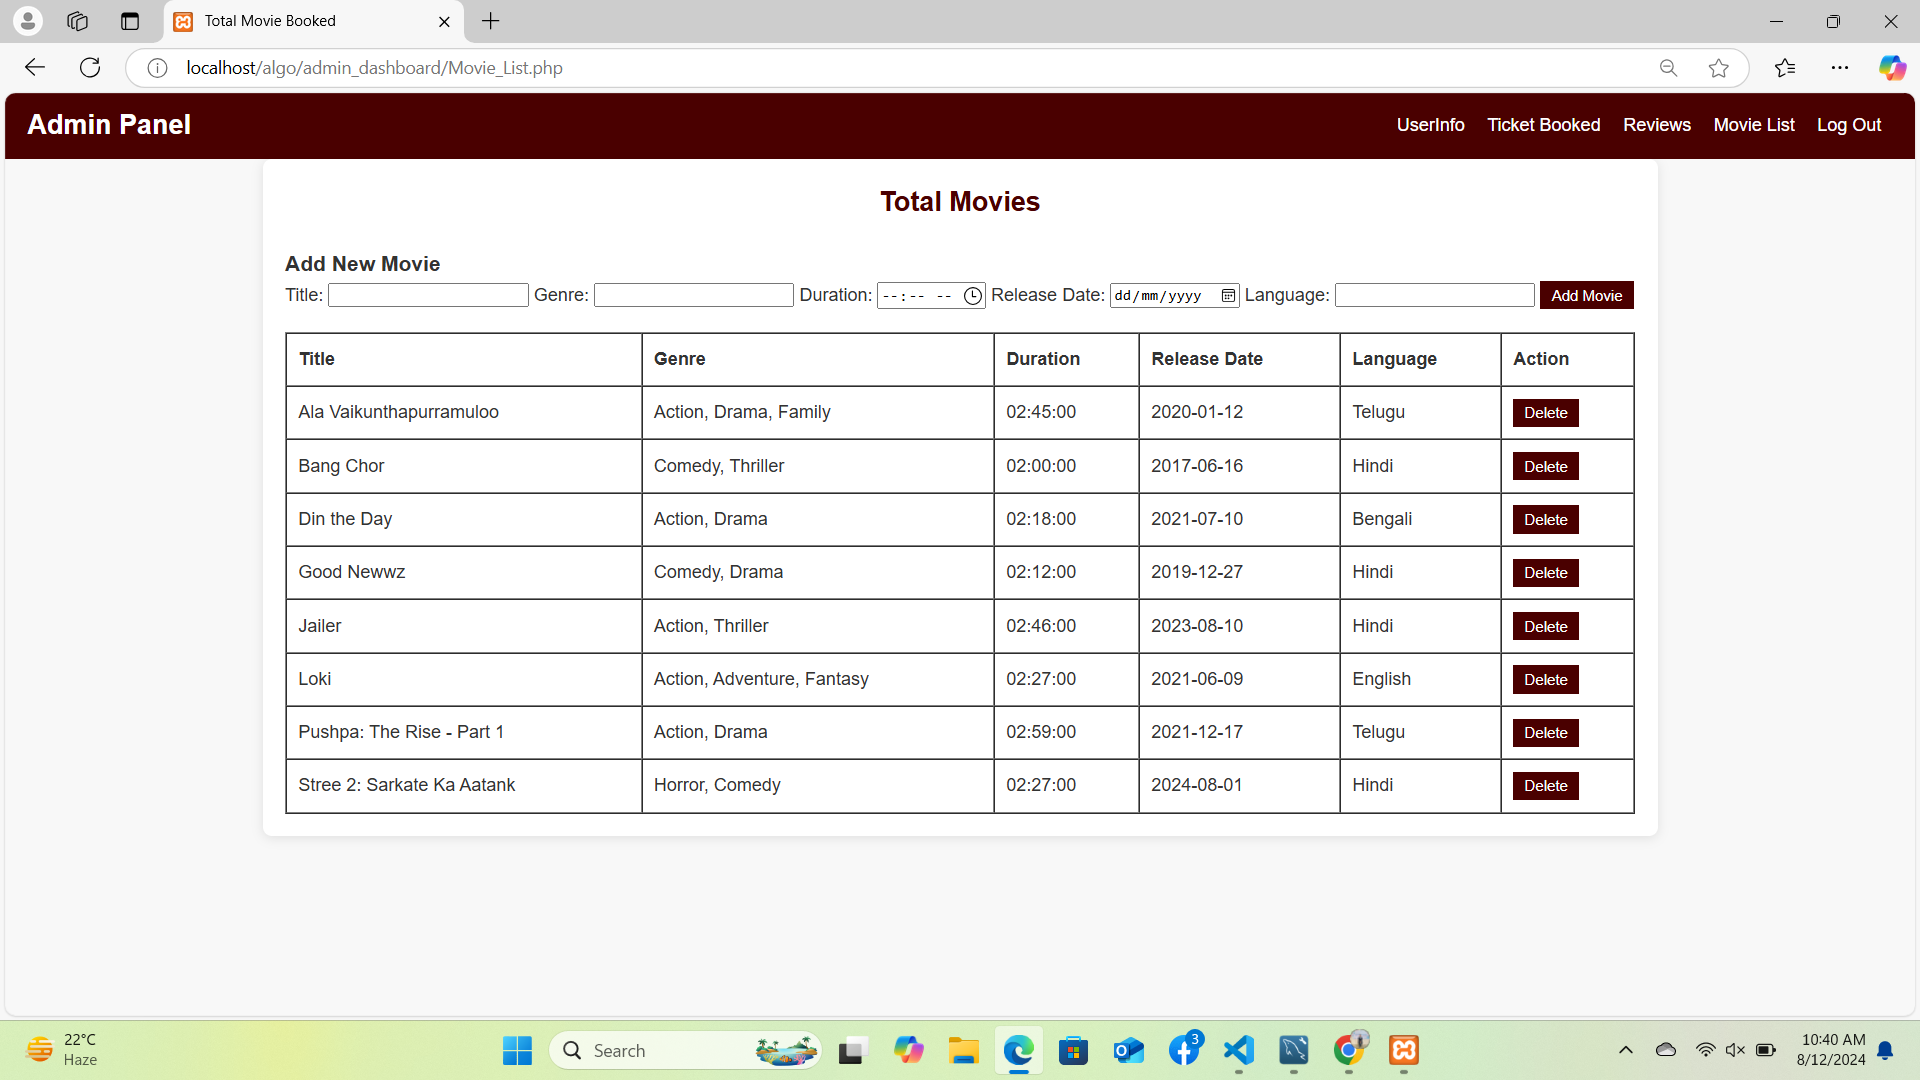
\includegraphics[width=\textwidth]{Photo13.png}
    \caption{Movie List}
    \label{fig:photo}
\end{figure}
\newpage






\newpage
\newpage


\begin{figure}[h!]
\section{ER Diagram}
    \centering
    \includegraphics[width=\textwidth]{erpic.png}
    \caption{Image Caption}
    \label{fig:photo06}
\end{figure}

\newpage



\clearpage




% Implementation
\section{Implementation} \label{sec:imp}

\subsection{SQL code}
Provide code snippets for each component of your system. For example, Listing~\ref{list:sql} shows an SQL query:

\begin{lstlisting}[caption={SQL Database Creation for Movie Management System}, label=list:sql, language=SQL, frame=single, basicstyle=\ttfamily\small, keywordstyle=\color{brown}, commentstyle=\color{gray}, stringstyle=\color{blue}]
-- Create database
CREATE DATABASE dbms;

-- Use the database
USE dbms;

-- Create AccountUser table
CREATE TABLE AccountUser (
    username VARCHAR(255) PRIMARY KEY,
    email VARCHAR(255) NOT NULL UNIQUE,
    name VARCHAR(255) NOT NULL,
    phone VARCHAR(15) NOT NULL,
    password VARCHAR(255) NOT NULL
);

-- Create Movie table
CREATE TABLE Movie (
    title VARCHAR(100) PRIMARY KEY,
    genre VARCHAR(50),
    duration TIME,
    release_date DATE,
    language VARCHAR(50)
);

-- Create MovieSession table
CREATE TABLE MovieSession (
    session_id INT AUTO_INCREMENT PRIMARY KEY,
    movie_title VARCHAR(100),
    session_time VARCHAR(100),
    FOREIGN KEY (movie_title) REFERENCES Movie(title) ON DELETE CASCADE
);

-- Create Review table
CREATE TABLE Review (
    review_id INT AUTO_INCREMENT PRIMARY KEY,
    username VARCHAR(255),
    movie_title VARCHAR(100),
    rating INT CHECK (rating BETWEEN 1 AND 10),
    comment TEXT,
    review_date DATETIME,
    FOREIGN KEY (username) REFERENCES AccountUser(username) ON DELETE CASCADE,
    FOREIGN KEY (movie_title) REFERENCES Movie(title) ON DELETE CASCADE
);

-- Create moviebooked table
CREATE TABLE moviebooked (
    username VARCHAR(255),
    movie_title VARCHAR(100),
    show_time VARCHAR(50),  -- Day, Afternoon, Evening, Night
    number_of_tickets INT,
    price VARCHAR(50),  -- Luxary, Premium, Regular
    seat_number INT AUTO_INCREMENT,
    purchase_date DATE,
    Payment_ID VARCHAR(50),
    PRIMARY KEY (seat_number),
    FOREIGN KEY (username) REFERENCES AccountUser(username) ON DELETE CASCADE,
    FOREIGN KEY (movie_title) REFERENCES Movie(title) ON DELETE CASCADE
);

-- Set auto increment behavior for seat_number based on price
DELIMITER //
CREATE TRIGGER set_seat_number BEFORE INSERT ON moviebooked
FOR EACH ROW
BEGIN
    IF NEW.price = 'Regular' THEN
        SET NEW.seat_number = (SELECT IFNULL(MAX(seat_number), 999) + 1 FROM moviebooked WHERE price = 'Regular');
    ELSEIF NEW.price = 'Premium' THEN
        SET NEW.seat_number = (SELECT IFNULL(MAX(seat_number), 1999) + 1 FROM moviebooked WHERE price = 'Premium');
    ELSEIF NEW.price = 'Luxary' THEN
        SET NEW.seat_number = (SELECT IFNULL(MAX(seat_number), 2999) + 1 FROM moviebooked WHERE price = 'Luxary');
    END IF;
END; //
DELIMITER ;

-- Insert Movies
INSERT INTO Movie (title, genre, duration, release_date, language)
VALUES 
('Loki', 'Action, Adventure, Fantasy', '02:27:00', '2021-06-09', 'English'),
('Stree 2: Sarkate Ka Aatank', 'Horror, Comedy', '02:27:00', '2024-08-01', 'Hindi'),
('Pushpa: The Rise - Part 1', 'Action, Drama', '02:59:00', '2021-12-17', 'Telugu'),
('Jailer', 'Action, Thriller', '02:46:00', '2023-08-10', 'Hindi'),
('Ala Vaikunthapurramuloo', 'Action, Drama, Family', '02:45:00', '2020-01-12', 'Telugu'),
('Good Newwz', 'Comedy, Drama', '02:12:00', '2019-12-27', 'Hindi'),
('Bang Chor', 'Comedy, Thriller', '02:00:00', '2017-06-16', 'Hindi'),
('Din the Day', 'Action, Drama', '02:18:00', '2021-07-10', 'Bengali');

-- Insert Movie Sessions for all movies
INSERT INTO MovieSession (movie_title, session_time)
VALUES 
('Loki', 'Day(12.00)'),
('Loki', 'After-Noon(3.00)'),
('Loki', 'Evening(6.00)'),
('Loki', 'Night(9.00)'),
('Stree 2: Sarkate Ka Aatank', 'Day(12.00)'),
('Stree 2: Sarkate Ka Aatank', 'After-Noon(3.00)'),
('Stree 2: Sarkate Ka Aatank', 'Evening(6.00)'),
('Stree 2: Sarkate Ka Aatank', 'Night(9.00)'),
('Pushpa: The Rise - Part 1', 'Day(12.00)'),
('Pushpa: The Rise - Part 1', 'After-Noon(3.00)'),
('Pushpa: The Rise - Part 1', 'Evening(6.00)'),
('Pushpa: The Rise - Part 1', 'Night(9.00)'),
('Jailer', 'Day(12.00)'),
('Jailer', 'After-Noon(3.00)'),
('Jailer', 'Evening(6.00)'),
('Jailer', 'Night(9.00)'),
('Ala Vaikunthapurramuloo', 'Day(12.00)'),
('Ala Vaikunthapurramuloo', 'After-Noon(3.00)'),
('Ala Vaikunthapurramuloo', 'Evening(6.00)'),
('Ala Vaikunthapurramuloo', 'Night(9.00)'),
('Good Newwz', 'Day(12.00)'),
('Good Newwz', 'After-Noon(3.00)'),
('Good Newwz', 'Evening(6.00)'),
('Good Newwz', 'Night(9.00)'),
('Bang Chor', 'Day(12.00)'),
('Bang Chor', 'After-Noon(3.00)'),
('Bang Chor', 'Evening(6.00)'),
('Bang Chor', 'Night(9.00)'),
('Din the Day', 'Day(12.00)'),
('Din the Day', 'After-Noon(3.00)'),
('Din the Day', 'Evening(6.00)'),
('Din the Day', 'Night(9.00)');
\end{lstlisting}


\subsection{Database Connection}
We have used \texttt{connection.php} to connect the database with the system. Listing 2 shows the database connection.

\begin{lstlisting}[language=PHP, caption={Database Connection}, label={lst:db_connect}]
<?php
$con = mysqli_connect("localhost", "root", "", "dbms")
    or die("Connection failed");
if (mysqli_connect_error()) {
    echo "Cannot Connect";
}
?>
\end{lstlisting}




\subsection{Create, Read, Update and Delete from Database}

\subsubsection{Fetch All Booked Movies for the Current User}
To retrieve all booked movies for the current user, the following SQL query is used:

\begin{lstlisting}[language=SQL, caption={Fetch All Booked Movies for the Current User}, label={lst:fetch_booked_movies}]
SELECT 
    moviebooked.seat_number, 
    moviebooked.movie_title, 
    moviebooked.show_time, 
    moviebooked.price, 
    moviebooked.purchase_date, 
    moviebooked.Payment_ID,
    moviebooked.number_of_tickets -- New column added
FROM moviebooked
WHERE moviebooked.username = ?
\end{lstlisting}

\subsubsection{Fetch All Reviews for the Current User}
To fetch all reviews written by the current user, the following query is used:

\begin{lstlisting}[language=SQL, caption={Fetch All Reviews for the Current User}, label={lst:fetch_reviews}]
SELECT 
    review.review_id, 
    review.movie_title, 
    review.rating, 
    review.comment, 
    review.review_date 
FROM review
WHERE review.username = ?
\end{lstlisting}

\subsubsection{Display User Data and Delete Action}
Here is the PHP code that fetches and displays user information, allowing an admin to delete a user:

\begin{lstlisting}[language=PHP, caption={Display User Data and Delete Action}, label={lst:user_delete_action}]
if ($result->num_rows > 0) {
    while ($row = $result->fetch_assoc()) {
        echo "<tr>
                <td>{$row['username']}</td>
                <td>{$row['email']}</td>
                <td>{$row['name']}</td>
                <td>{$row['phone']}</td>
                <td>
                    <a href='AboutUser.php?delete={$row['username']}' onclick='return confirm(\"Are you sure you want to delete this user?\");'>
                        <button class='actions'>Delete</button>
                    </a>
                </td>
              </tr>";
    }
} else {
    echo "<tr><td colspan='5'>No users found</td></tr>";
}
\end{lstlisting}

\subsubsection{Fetch Booking Data}
To fetch booking data, the following SQL query is used:

\begin{lstlisting}[language=SQL, caption={Fetch Booking Data}, label={lst:fetch_booking_data}]
SELECT 
    moviebooked.movie_title AS title, 
    moviebooked.username AS user, 
    SUM(moviebooked.number_of_tickets) AS total_tickets, 
    moviebooked.show_time, 
    GROUP_CONCAT(DISTINCT moviebooked.Payment_ID SEPARATOR ', ') AS payment_ids
FROM moviebooked 
GROUP BY moviebooked.movie_title, moviebooked.username, moviebooked.show_time;
\end{lstlisting}

\subsubsection{Delete Booking Data}
To delete a booking record from the database, the following query is used:

\begin{lstlisting}[language=SQL, caption={Delete Booking Data}, label={lst:delete_booking_data}]
DELETE FROM moviebooked 
WHERE movie_title = '$title' 
    AND username = '$username' 
    AND show_time = '$show_time';
\end{lstlisting}

\subsubsection{Display Booking Data and Delete Action}
Here is the PHP code that fetches booking data and allows an admin to delete a booking:

\begin{lstlisting}[language=PHP, caption={Display Booking Data and Delete Action}, label={lst:booking_delete_action}]
if ($result->num_rows > 0) {
    while ($row = $result->fetch_assoc()) {
        echo "<tr>
            <td>" . htmlspecialchars($row['title']) . "</td>
            <td>" . htmlspecialchars($row['user']) . "</td>
            <td>" . htmlspecialchars($row['total_tickets']) . "</td>
            <td>" . htmlspecialchars($row['show_time']) . "</td>
            <td>" . htmlspecialchars($row['payment_ids']) . "</td> <!-- Display Payment IDs -->
            <td>
                <form method='POST' action='TotalMovieBooked.php'>
                    <input type='hidden' name='title' value='" . htmlspecialchars($row['title']) . "'>
                    <input type='hidden' name='username' value='" . htmlspecialchars($row['user']) . "'>
                    <input type='hidden' name='show_time' value='" . htmlspecialchars($row['show_time']) . "'>
                    <button type='submit' name='delete' style='background-color: #4A0000; color: white; border: none; padding: 5px 10px; cursor: pointer;'>Delete</button>
                </form>
            </td>
        </tr>";
    }
} else {
    echo "<tr><td colspan='6'>No bookings found.</td></tr>";
}
\end{lstlisting}













\clearpage




% Validation
\section{Validation} \label{sec:val}

The validation of the \textbf{Movie Management System} project was conducted to ensure that the system met the expectations of users and performed optimally. The validation process included measuring user satisfaction, performing usability tests, gathering feedback, and comparing the system’s performance with alternative platforms.

\subsection{User Satisfaction Measurement}

User satisfaction was measured through a combination of user testing, surveys, and direct feedback. A group of target users was invited to interact with the \textbf{Movie Management System} during different stages of development. After using the system, users were asked to complete surveys that assessed their satisfaction with various aspects of the system, including:

\begin{itemize}
    \item \textbf{Ease of Use}: How easy it was to navigate through the website, sign up, and interact with features like movie listing, review submission, and reading reviews.
    \item \textbf{Design and Aesthetics}: Users rated the visual appeal of the interface, the organization of the content, and the responsiveness of the website.
    \item \textbf{Functionality}: How well the website functions, including movie search, review submission, and ratings system.
    \item \textbf{Performance}: How quickly the website loaded pages, especially the movie list and review submission forms.
\end{itemize}

The results from the surveys were used to make improvements to the system, ensuring that the needs and preferences of the users were met.

\subsection{User Manual}

The user manual provides step-by-step instructions on how to use the \textbf{Movie Management System} effectively. Below are the detailed instructions for various tasks:

\begin{itemize}
    \item \textbf{Sign Up}:
    \begin{enumerate}
        \item Open the Movie Management System homepage.
        \item Click on the "Sign Up" button located in the top right corner or the "Join Us" button at the middle of the page.
        \item Fill in the registration form with the following details:
        \begin{itemize}
            \item \textbf{Username}: Choose a unique username.
            \item \textbf{Email}: Provide a valid email address.
            \item \textbf{Password}: Set a secure password.
        \end{itemize}
        \item Click on the "Submit" button to complete the registration process.
        \item Once registered, you can log in using your credentials.
    \end{enumerate}
    
    \item \textbf{Login}:
    \begin{enumerate}
        \item On the homepage, click on the "Login" button located in the top right corner.
        \item Enter your registered \textbf{Username} and \textbf{Password}.
        \item Click "Login" to access your user dashboard.
    \end{enumerate}

    \item \textbf{Viewing Movie List}:
    \begin{enumerate}
        \item After logging in, you will be redirected to your user dashboard.
        \item On the sidebar or navbar, click on the "Movie List" section to view all available movies.
        \item Click on any movie title to view more details, such as the genre, description, and cast.
    \end{enumerate}

    \item \textbf{Submitting Reviews and Ratings}:
    \begin{enumerate}
        \item In your user dashboard, select a movie from the list or search for a movie by name.
        \item Fill in the review form:
        \begin{itemize}
            \item \textbf{Rating}: Assign a rating from 1 to 10.
            \item \textbf{Review}: Write your thoughts and feedback about the movie.
        \end{itemize}
        \item Click the "Submit Review" button to post your review.
        \item Your review will appear on the movie's page and can be seen by other users.
    \end{enumerate}

    \item \textbf{Reading Reviews}:
    \begin{enumerate}
        \item Click on the "Reviews" button on the top right corner (only available after logging in).
        \item You can search for reviews by movie name to see the reviews for a specific movie.
    \end{enumerate}
\end{itemize}

Through user testing, feedback collection, and performance evaluation, the \textbf{Movie Management System} was validated to meet the expectations of its users. The system's performance in terms of response time, stability, and usability is competitive with other platforms in the market.


\clearpage



% Software Deployment
\section{Software Deployment} \label{sec:sd}

The deployment of the \textbf{Movie Management System} involves making the application accessible to users by hosting it on a web server. Below is a description of the steps involved in the deployment process, including the tools used, the environment setup, and deployment steps.

\subsection{Development Environment}
The development of the \textbf{Movie Management System} project was carried out using the following technologies:
\begin{itemize}
    \item \textbf{Frontend}: HTML, CSS
    \item \textbf{Backend}: PHP
    \item \textbf{Database}: MySQL
\end{itemize}

The project was initially developed and tested locally using a local server environment, with XAMPP for Windows, which includes Apache (for the web server) and MySQL (for the database). The local development environment allowed easy testing and debugging before moving the application to the production server.

\subsection{Production Environment}
For the production deployment of the \textbf{Movie Management System} project, the following steps were followed:

\begin{enumerate}
    \item \textbf{Choosing the Hosting Service}:
    \begin{itemize}
        \item A shared hosting service or cloud provider (XAMPP) was chosen for deployment.
        \item The server supports PHP and MySQL to meet the technical requirements of the \textbf{Movie Management System} application.
    \end{itemize}
    
    \item \textbf{Setting Up the Server}:
    \begin{itemize}
        \item Install the required software: Apache, PHP, and MySQL.
        \item Configure the Apache server to serve the application’s files.
        \item Set up a MySQL database with the necessary schemas and tables.
    \end{itemize}
    
    \item \textbf{Database Migration}:
    \begin{itemize}
        \item Export the local database (using phpMyAdmin or MySQL command line).
        \item Import the database to the production MySQL server using phpMyAdmin or command line.
    \end{itemize}
    
    \item \textbf{File Upload}:
    \begin{itemize}
        \item The application files (PHP scripts, CSS, HTML files, images) were uploaded to the production server.
        \item FTP or SSH protocols were used to transfer files from the local machine to the server.
    \end{itemize}
    
    \item \textbf{Configuration Adjustments}:
    \begin{itemize}
        \item Configuration files (e.g., database connection settings) were adjusted to match the production environment.
        \item Paths for assets and files were updated to reflect the directory structure on the production server.
    \end{itemize}
    
    \item \textbf{Testing the Deployed Application}:
    \begin{itemize}
        \item After deployment, thorough testing was done to ensure that the application was fully functional in the live environment.
        \item This included testing user registrations, logins, movie listings, reviews, and admin functionality.
    \end{itemize}
    
    \item \textbf{Setting Up Security Measures}:
    \begin{itemize}
        \item SSL certificates were installed for secure connections (HTTPS).
        \item Security settings for PHP (e.g., disabling dangerous functions) were configured.
    \end{itemize}
\end{enumerate}

\subsection{Deployment Tools}
The following tools were used during deployment:
\begin{itemize}
    \item \textbf{FTP/SFTP}: For transferring files between local and production environments.
    \item \textbf{phpMyAdmin}: For managing the MySQL database in both development and production environments.
    \item \textbf{SSL Certificates}: For securing data transmitted between users and the server.
    \item \textbf{SSH}: For remote server access and management.
\end{itemize}

\subsection{Post-Deployment Tasks}
Once \textbf{Movie Management System} was deployed, several tasks were performed to ensure its smooth operation:
\begin{itemize}
    \item \textbf{Monitoring}: Regular monitoring of server performance and application usage was done using tools like Google Analytics and server logs.
    \item \textbf{Backup}: A backup system was set up to create periodic backups of both the application files and the MySQL database.
    \item \textbf{Bug Fixes and Updates}: Post-deployment bug fixes and feature updates were implemented as needed, and the application was regularly updated to ensure security and performance improvements.
\end{itemize}



\clearpage




% Conclusion and Future Work
\section{Conclusion and Future Work} \label{sec:cfw}

\subsection{Conclusion}
The \textbf{Movie Management System} project successfully addresses the need for a centralized platform where users can explore movie content, share their experiences through reviews, and rate the movies they have watched. The platform allows users to register, log in, browse a movie list, and submit reviews and ratings. Admins have the ability to manage users, update the movie list, and moderate reviews, ensuring smooth operation and content management on the platform.

The solution provides a user-friendly interface for movie enthusiasts to interact with the community, rate movies, and get personalized recommendations. By leveraging technologies such as PHP, MySQL, HTML, and CSS, we were able to create a functional and responsive application that serves both individual users and administrative needs.

\subsection{Significance}
The \textbf{Movie Management System} serves as a valuable platform for movie lovers to express their opinions, discover new content, and engage with like-minded individuals. It allows users to rate and review movies, helping other users make informed decisions on what to watch. Additionally, the admin functionality ensures proper management of the content and users, maintaining the integrity of the platform.

The system also demonstrates a solid application of full-stack development practices, providing a real-world solution for handling user interactions, data management, and administration through a web-based interface.

\subsection{Limitations}
While the \textbf{Movie Management System} offers a robust set of features, there are a few limitations:
\begin{itemize}
    \item \textbf{No Reset Password Feature}: Users are currently unable to reset their passwords if they forget them. This could be a significant limitation in terms of user account recovery.
    \item \textbf{No Sorting or Filtering Options}: The movie list lacks sorting or filtering features, such as sorting by rating, genre, or popularity. This would enhance the user experience by making it easier to navigate the content.
    \item \textbf{Limited User Interaction}: Currently, there is no social interaction feature (e.g., comments on reviews or a discussion forum), which could further engage users in discussions about movies.
    \item \textbf{Lack of Mobile Responsiveness}: The platform is not fully optimized for mobile devices, which may limit its accessibility for users on smartphones or tablets.
\end{itemize}

\subsection{Future Work}
The following improvements and new features are planned for future versions of the \textbf{Movie Management System}:
\begin{itemize}
    \item \textbf{Password Reset Feature}: Implement a password recovery mechanism to allow users to reset their passwords securely.
    \item \textbf{Sorting and Filtering Options}: Add sorting and filtering options to the movie list, enabling users to sort by rating, genre, release year, and other relevant criteria.
    \item \textbf{User Interaction Features}: Add features such as the ability to comment on reviews, follow other users, or engage in discussions, fostering a stronger sense of community.
    \item \textbf{Mobile Optimization}: Enhance the responsiveness of the website to ensure it is fully functional on mobile devices, providing a seamless user experience across different platforms.
    \item \textbf{Movie Recommendation System}: Develop an algorithm that suggests movies to users based on their ratings and reviews, improving personalization and user engagement.
    \item \textbf{Advanced Admin Controls}: Enhance admin functionalities by adding features such as managing comments, banning inappropriate content, and more granular user roles.
\end{itemize}

By addressing these limitations and introducing new features, the \textbf{Movie Management System} has the potential to evolve into a more comprehensive and interactive platform for movie fans worldwide.



\clearpage




\section{References}
\begin{enumerate}
    \item \textbf{Zoom}. \textit{Source:} \url{https://en.wikipedia.org/wiki/Zoom_Video_Communications}
    \item \textbf{Trello}. \textit{Source:} \url{https://en.wikipedia.org/wiki/Trello}
    \item \textbf{GitHub}. \textit{Source:} \url{https://en.wikipedia.org/wiki/GitHub}
    \item \textbf{VS-Code}. \textit{Source:} \url{https://en.wikipedia.org/wiki/Visual_Studio_Code#:~:text=Visual%20Studio%20Code%2C%20also%20commonly,code%20refactoring%2C%20and%20embedded%20Git.}
    \item \textbf{XAMPP}. \textit{Source:} \url{https://en.wikipedia.org/wiki/XAMPP}
    \item \textbf{LATEX}. \textit{Source:} \url{https://en.wikipedia.org/wiki/LaTeX}
    \item \textbf{Draw.io}. \textit{Source:} \url{https://en.wiki.bluespice.com/wiki/Manual:Extension/DrawioEditor}
    \item \textbf{Canva}. \textit{Source:} \url{https://en.wikipedia.org/wiki/Canva}
    \item \textbf{First Normal Form}. \textit{Source:} \url{https://en.wikipedia.org/wiki/Second_normal_form}
    \item \textbf{Second Normal Form}. \textit{Source:} \url{https://en.wikipedia.org/wiki/First_normal_form}
    \item \textbf{A. Silberschatz, H.F. Korth, S. Sudarshan et al.}, Third Normal Form, Vol.4, McGraw-Hill New York, 1997.
    \item \textbf{A. Silberschatz, H.F. Korth, S. Sudarshan et al.}, Boyce–Codd Normal Form, Vol.4, McGraw-Hill New York, 1997.
\end{enumerate}

\end{document}